% IEEE Access manuscript. Build: python paper/build_latex.py
% Every number is written \val{<claim id>} and printed from paper/numbers.csv; claims that
% print no number carry a comment naming their claim id. Do not type results into this file.
\documentclass[journal]{IEEEtran}
\usepackage[T1]{fontenc}
\usepackage[utf8]{inputenc}
\usepackage{newtxtext,newtxmath}
\usepackage{amsmath}
\usepackage{graphicx}
\usepackage{booktabs,array,makecell}
\usepackage{cite}
\usepackage{algorithm}
\usepackage{algpseudocode}
\usepackage{url}
\usepackage{textcomp}
\usepackage{stfloats}
\usepackage[hidelinks]{hyperref}

% AUTO-GENERATED by paper/build_latex.py from paper/numbers.csv. Do not edit.
\makeatletter
\@namedef{val@campaign_runs_total}{180}% analysis/final/run_level_data.csv
\@namedef{val@campaign_architectures}{2}% analysis/final/run_level_data.csv
\@namedef{val@campaign_cells}{36}% analysis/final/run_level_data.csv
\@namedef{val@campaign_reps_per_cell}{5}% analysis/final/run_level_data.csv
\@namedef{val@campaign_fault_types}{2}% analysis/final/run_level_data.csv
\@namedef{val@campaign_runs_failed}{0}% analysis/final/run_level_data.csv
\@namedef{val@campaign_runs_censored}{0}% analysis/final/run_level_data.csv
\@namedef{val@campaign_censoring_rate_pct}{0.0}% analysis/final/run_level_data.csv
\@namedef{val@campaign_gateway_runs}{0}% analysis/final/run_level_data.csv
\@namedef{val@sn_runs}{110}% analysis/final/run_level_data.csv
\@namedef{val@sn_services}{11}% analysis/final/run_level_data.csv
\@namedef{val@hr_runs}{70}% analysis/final/run_level_data.csv
\@namedef{val@hr_services}{7}% analysis/final/run_level_data.csv
\@namedef{val@campaign_start_utc}{2026-09-26 05:02}% analysis/final/run_level_data.csv
\@namedef{val@campaign_end_utc}{2026-09-26 13:35}% analysis/final/run_level_data.csv
\@namedef{val@campaign_duration_hours}{8.5}% analysis/final/run_level_data.csv
\@namedef{val@integrity_checks_total}{10}% analysis/final/integrity_checks.csv
\@namedef{val@integrity_checks_passed}{10}% analysis/final/integrity_checks.csv
\@namedef{val@primary_rho}{0.785}% analysis/final/confirmatory_family_kill.csv
\@namedef{val@primary_rho_full}{0.785119}% analysis/final/confirmatory_family_kill.csv
\@namedef{val@primary_ci_lo}{0.000}% analysis/final/confirmatory_family_kill.csv
\@namedef{val@primary_ci_hi}{1.000}% analysis/final/confirmatory_family_kill.csv
\@namedef{val@primary_ci_method}{BCa}% analysis/final/confirmatory_family_kill.csv
\@namedef{val@primary_n_services}{11}% analysis/final/confirmatory_family_kill.csv
\@namedef{val@primary_p_locked}{0.0080}% analysis/final/confirmatory_family_kill.csv
\@namedef{val@primary_p_bh_locked}{0.3451}% analysis/final/confirmatory_family_kill.csv
\@namedef{val@primary_significant}{no}% analysis/final/confirmatory_family_kill.csv
\@namedef{val@primary_p_exact}{0.006926}% analysis/final/exact_p_supplement.csv
\@namedef{val@primary_p_exact_arrangements}{9,240}% analysis/final/exact_p_supplement.csv
\@namedef{val@primary_p_bh_exact}{0.3048}% analysis/final/exact_p_supplement.csv
\@namedef{val@primary_significant_exact}{no}% analysis/final/exact_p_supplement.csv
\@namedef{val@exact_tests_refined}{43}% analysis/final/exact_p_supplement.csv
\@namedef{val@conf_family_size}{44}% analysis/final/confirmatory_family_kill.csv
\@namedef{val@conf_family_defined}{44}% analysis/final/confirmatory_family_kill.csv
\@namedef{val@conf_family_significant}{0}% analysis/final/confirmatory_family_kill.csv
\@namedef{val@conf_best_raw_p}{0.0080}% analysis/final/confirmatory_family_kill.csv
\@namedef{val@conf_best_bh_p}{0.3451}% analysis/final/confirmatory_family_kill.csv
\@namedef{val@conf_best_predictor}{ancestor\_count}% analysis/final/confirmatory_family_kill.csv
\@namedef{val@repl_family_size}{44}% analysis/final/replication_family_latency.csv
\@namedef{val@repl_family_defined}{44}% analysis/final/replication_family_latency.csv
\@namedef{val@repl_family_significant}{0}% analysis/final/replication_family_latency.csv
\@namedef{val@repl_best_raw_p}{0.0076}% analysis/final/replication_family_latency.csv
\@namedef{val@repl_best_bh_p}{0.1848}% analysis/final/replication_family_latency.csv
\@namedef{val@repl_best_predictor}{ancestor\_count}% analysis/final/replication_family_latency.csv
\@namedef{val@fdr_q}{0.05}% analysis/final/confirmatory_family_kill.csv
\@namedef{val@trec_conf_tests}{22}% analysis/final/confirmatory_family_kill.csv
\@namedef{val@trec_conf_significant}{0}% analysis/final/confirmatory_family_kill.csv
\@namedef{val@trec_conf_logrank_undefined}{10}% analysis/final/confirmatory_family_kill.csv
\@namedef{val@trec_conf_sn_ancestor_rho}{\ensuremath{-}0.356}% analysis/final/confirmatory_family_kill.csv
\@namedef{val@trec_conf_sn_ancestor_p}{0.2807}% analysis/final/confirmatory_family_kill.csv
\@namedef{val@trec_conf_sn_ancestor_bh_p}{0.9264}% analysis/final/confirmatory_family_kill.csv
\@namedef{val@trec_conf_sn_ancestor_logrank_p}{0.5154}% analysis/final/confirmatory_family_kill.csv
\@namedef{val@trec_conf_sn_ancestor_cox_run_hr}{1.173}% analysis/final/confirmatory_family_kill.csv
\@namedef{val@trec_conf_sn_ancestor_cox_run_ci_lo}{0.876}% analysis/final/confirmatory_family_kill.csv
\@namedef{val@trec_conf_sn_ancestor_cox_run_ci_hi}{1.570}% analysis/final/confirmatory_family_kill.csv
\@namedef{val@trec_conf_sn_ancestor_cox_run_p}{0.2836}% analysis/final/confirmatory_family_kill.csv
\@namedef{val@trec_conf_sn_ancestor_cox_service_hr}{1.479}% analysis/final/confirmatory_family_kill.csv
\@namedef{val@trec_conf_sn_ancestor_cox_service_ci_lo}{0.688}% analysis/final/confirmatory_family_kill.csv
\@namedef{val@trec_conf_sn_ancestor_cox_service_ci_hi}{3.181}% analysis/final/confirmatory_family_kill.csv
\@namedef{val@trec_conf_sn_ancestor_cox_service_p}{0.3163}% analysis/final/confirmatory_family_kill.csv
\@namedef{val@trec_conf_hr_ancestor_rho}{\ensuremath{-}0.158}% analysis/final/confirmatory_family_kill.csv
\@namedef{val@trec_conf_hr_ancestor_p}{0.8571}% analysis/final/confirmatory_family_kill.csv
\@namedef{val@trec_conf_hr_ancestor_bh_p}{0.9925}% analysis/final/confirmatory_family_kill.csv
\@namedef{val@trec_conf_hr_ancestor_cox_run_hr}{1.522}% analysis/final/confirmatory_family_kill.csv
\@namedef{val@trec_conf_hr_ancestor_cox_run_ci_lo}{1.067}% analysis/final/confirmatory_family_kill.csv
\@namedef{val@trec_conf_hr_ancestor_cox_run_ci_hi}{2.171}% analysis/final/confirmatory_family_kill.csv
\@namedef{val@trec_conf_hr_ancestor_cox_run_p}{0.0204}% analysis/final/confirmatory_family_kill.csv
\@namedef{val@trec_conf_hr_ancestor_cox_service_hr}{2.179}% analysis/final/confirmatory_family_kill.csv
\@namedef{val@trec_conf_hr_ancestor_cox_service_ci_lo}{0.302}% analysis/final/confirmatory_family_kill.csv
\@namedef{val@trec_conf_hr_ancestor_cox_service_ci_hi}{15.722}% analysis/final/confirmatory_family_kill.csv
\@namedef{val@trec_conf_hr_ancestor_cox_service_p}{0.4399}% analysis/final/confirmatory_family_kill.csv
\@namedef{val@trec_conf_sn_hybrid_rho}{0.098}% analysis/final/confirmatory_family_kill.csv
\@namedef{val@trec_conf_sn_hybrid_p}{0.7699}% analysis/final/confirmatory_family_kill.csv
\@namedef{val@trec_conf_sn_hybrid_bh_p}{0.9925}% analysis/final/confirmatory_family_kill.csv
\@namedef{val@trec_conf_sn_hybrid_logrank_p}{0.2099}% analysis/final/confirmatory_family_kill.csv
\@namedef{val@trec_conf_hr_hybrid_rho}{0.204}% analysis/final/confirmatory_family_kill.csv
\@namedef{val@trec_conf_hr_hybrid_p}{0.8571}% analysis/final/confirmatory_family_kill.csv
\@namedef{val@trec_conf_hr_hybrid_bh_p}{0.9925}% analysis/final/confirmatory_family_kill.csv
\@namedef{val@trec_repl_tests}{22}% analysis/final/replication_family_latency.csv
\@namedef{val@trec_repl_significant}{0}% analysis/final/replication_family_latency.csv
\@namedef{val@trec_repl_logrank_undefined}{10}% analysis/final/replication_family_latency.csv
\@namedef{val@trec_repl_sn_ancestor_rho}{\ensuremath{-}0.060}% analysis/final/replication_family_latency.csv
\@namedef{val@trec_repl_sn_ancestor_p}{0.8647}% analysis/final/replication_family_latency.csv
\@namedef{val@trec_repl_sn_ancestor_bh_p}{1.0000}% analysis/final/replication_family_latency.csv
\@namedef{val@trec_repl_sn_ancestor_logrank_p}{0.5561}% analysis/final/replication_family_latency.csv
\@namedef{val@trec_repl_sn_ancestor_cox_run_hr}{0.998}% analysis/final/replication_family_latency.csv
\@namedef{val@trec_repl_sn_ancestor_cox_run_ci_lo}{0.816}% analysis/final/replication_family_latency.csv
\@namedef{val@trec_repl_sn_ancestor_cox_run_ci_hi}{1.221}% analysis/final/replication_family_latency.csv
\@namedef{val@trec_repl_sn_ancestor_cox_run_p}{0.9859}% analysis/final/replication_family_latency.csv
\@namedef{val@trec_repl_sn_ancestor_cox_service_hr}{1.184}% analysis/final/replication_family_latency.csv
\@namedef{val@trec_repl_sn_ancestor_cox_service_ci_lo}{0.627}% analysis/final/replication_family_latency.csv
\@namedef{val@trec_repl_sn_ancestor_cox_service_ci_hi}{2.236}% analysis/final/replication_family_latency.csv
\@namedef{val@trec_repl_sn_ancestor_cox_service_p}{0.6018}% analysis/final/replication_family_latency.csv
\@namedef{val@trec_repl_hr_ancestor_rho}{\ensuremath{-}0.158}% analysis/final/replication_family_latency.csv
\@namedef{val@trec_repl_hr_ancestor_p}{0.8571}% analysis/final/replication_family_latency.csv
\@namedef{val@trec_repl_hr_ancestor_bh_p}{1.0000}% analysis/final/replication_family_latency.csv
\@namedef{val@trec_repl_hr_ancestor_cox_run_hr}{0.882}% analysis/final/replication_family_latency.csv
\@namedef{val@trec_repl_hr_ancestor_cox_run_ci_lo}{0.578}% analysis/final/replication_family_latency.csv
\@namedef{val@trec_repl_hr_ancestor_cox_run_ci_hi}{1.346}% analysis/final/replication_family_latency.csv
\@namedef{val@trec_repl_hr_ancestor_cox_run_p}{0.5609}% analysis/final/replication_family_latency.csv
\@namedef{val@trec_repl_hr_ancestor_cox_service_hr}{2.179}% analysis/final/replication_family_latency.csv
\@namedef{val@trec_repl_hr_ancestor_cox_service_ci_lo}{0.302}% analysis/final/replication_family_latency.csv
\@namedef{val@trec_repl_hr_ancestor_cox_service_ci_hi}{15.722}% analysis/final/replication_family_latency.csv
\@namedef{val@trec_repl_hr_ancestor_cox_service_p}{0.4399}% analysis/final/replication_family_latency.csv
\@namedef{val@trec_repl_sn_hybrid_rho}{0.767}% analysis/final/replication_family_latency.csv
\@namedef{val@trec_repl_sn_hybrid_p}{0.0084}% analysis/final/replication_family_latency.csv
\@namedef{val@trec_repl_sn_hybrid_bh_p}{0.1848}% analysis/final/replication_family_latency.csv
\@namedef{val@trec_repl_sn_hybrid_logrank_p}{0.1099}% analysis/final/replication_family_latency.csv
\@namedef{val@trec_repl_hr_hybrid_rho}{0.408}% analysis/final/replication_family_latency.csv
\@namedef{val@trec_repl_hr_hybrid_p}{0.5714}% analysis/final/replication_family_latency.csv
\@namedef{val@trec_repl_hr_hybrid_bh_p}{0.8111}% analysis/final/replication_family_latency.csv
\@namedef{val@expl_attempted}{154}% analysis/final/exploratory_family.csv
\@namedef{val@expl_testable}{66}% analysis/final/exploratory_family.csv
\@namedef{val@expl_undefined}{88}% analysis/final/exploratory_family.csv
\@namedef{val@expl_significant}{2}% analysis/final/exploratory_family.csv
\@namedef{val@expl_sig_hybrid_criticality_rho}{0.949}% analysis/final/exploratory_family.csv
\@namedef{val@expl_sig_hybrid_criticality_bh_p}{0.0033}% analysis/final/exploratory_family.csv
\@namedef{val@expl_sig_degree_rho}{0.953}% analysis/final/exploratory_family.csv
\@namedef{val@expl_sig_degree_bh_p}{0.0033}% analysis/final/exploratory_family.csv
\@namedef{val@h1b_sn_kill_rho}{\ensuremath{-}0.144}% analysis/final/h1b_hybrid_metric.csv
\@namedef{val@h1b_sn_kill_ci_lo}{\ensuremath{-}0.810}% analysis/final/h1b_hybrid_metric.csv
\@namedef{val@h1b_sn_kill_ci_hi}{0.698}% analysis/final/h1b_hybrid_metric.csv
\@namedef{val@h1b_sn_kill_p}{0.6688}% analysis/final/h1b_hybrid_metric.csv
\@namedef{val@h1b_sn_kill_bh_p}{0.9925}% analysis/final/h1b_hybrid_metric.csv
\@namedef{val@h1b_hr_kill_rho}{\ensuremath{-}0.258}% analysis/final/h1b_hybrid_metric.csv
\@namedef{val@h1b_hr_kill_ci_lo}{\ensuremath{-}0.730}% analysis/final/h1b_hybrid_metric.csv
\@namedef{val@h1b_hr_kill_ci_hi}{\ensuremath{-}0.167}% analysis/final/h1b_hybrid_metric.csv
\@namedef{val@h1b_hr_kill_p}{1.0000}% analysis/final/h1b_hybrid_metric.csv
\@namedef{val@h1b_hr_kill_bh_p}{1.0000}% analysis/final/h1b_hybrid_metric.csv
\@namedef{val@h1b_sn_latency_rho}{\ensuremath{-}0.144}% analysis/final/h1b_hybrid_metric.csv
\@namedef{val@h1b_sn_latency_ci_lo}{\ensuremath{-}0.805}% analysis/final/h1b_hybrid_metric.csv
\@namedef{val@h1b_sn_latency_ci_hi}{0.713}% analysis/final/h1b_hybrid_metric.csv
\@namedef{val@h1b_sn_latency_p}{0.6656}% analysis/final/h1b_hybrid_metric.csv
\@namedef{val@h1b_sn_latency_bh_p}{0.9152}% analysis/final/h1b_hybrid_metric.csv
\@namedef{val@h1b_hr_latency_rho}{\ensuremath{-}0.258}% analysis/final/h1b_hybrid_metric.csv
\@namedef{val@h1b_hr_latency_ci_lo}{\ensuremath{-}0.750}% analysis/final/h1b_hybrid_metric.csv
\@namedef{val@h1b_hr_latency_ci_hi}{\ensuremath{-}0.167}% analysis/final/h1b_hybrid_metric.csv
\@namedef{val@h1b_hr_latency_p}{1.0000}% analysis/final/h1b_hybrid_metric.csv
\@namedef{val@h1b_hr_latency_bh_p}{1.0000}% analysis/final/h1b_hybrid_metric.csv
\@namedef{val@h1b_all_negative}{yes}% analysis/final/h1b_hybrid_metric.csv
\@namedef{val@h1b_any_distinguishable}{no}% analysis/final/h1b_hybrid_metric.csv
\@namedef{val@h1b_cells}{4}% analysis/final/h1b_hybrid_metric.csv
\@namedef{val@saturation_sn_kill_run}{0.909}% analysis/final/ancestor_saturation.csv
\@namedef{val@saturation_sn_kill_service}{0.909}% analysis/final/ancestor_saturation.csv
\@namedef{val@saturation_sn_kill_tautological}{no}% analysis/final/ancestor_saturation.csv
\@namedef{val@saturation_sn_latency_run}{0.891}% analysis/final/ancestor_saturation.csv
\@namedef{val@saturation_sn_latency_service}{0.909}% analysis/final/ancestor_saturation.csv
\@namedef{val@saturation_sn_latency_tautological}{no}% analysis/final/ancestor_saturation.csv
\@namedef{val@saturation_hr_kill_run}{1.000}% analysis/final/ancestor_saturation.csv
\@namedef{val@saturation_hr_kill_service}{1.000}% analysis/final/ancestor_saturation.csv
\@namedef{val@saturation_hr_kill_tautological}{yes}% analysis/final/ancestor_saturation.csv
\@namedef{val@saturation_hr_latency_run}{1.000}% analysis/final/ancestor_saturation.csv
\@namedef{val@saturation_hr_latency_service}{1.000}% analysis/final/ancestor_saturation.csv
\@namedef{val@saturation_hr_latency_tautological}{yes}% analysis/final/ancestor_saturation.csv
\@namedef{val@composepost_kill_mean}{1.0}% analysis/final/compose_post_service.csv
\@namedef{val@composepost_kill_min}{1}% analysis/final/compose_post_service.csv
\@namedef{val@composepost_kill_max}{1}% analysis/final/compose_post_service.csv
\@namedef{val@composepost_kill_reps}{5}% analysis/final/compose_post_service.csv
\@namedef{val@composepost_latency_mean}{1.0}% analysis/final/compose_post_service.csv
\@namedef{val@composepost_latency_min}{1}% analysis/final/compose_post_service.csv
\@namedef{val@composepost_latency_max}{1}% analysis/final/compose_post_service.csv
\@namedef{val@composepost_latency_reps}{5}% analysis/final/compose_post_service.csv
\@namedef{val@composepost_rank_ancestor_count}{11}% analysis/final/compose_post_service.csv
\@namedef{val@composepost_rank_hybrid}{1}% analysis/final/compose_post_service.csv
\@namedef{val@composepost_set_size}{11}% analysis/final/compose_post_service.csv
\@namedef{val@composepost_ancestor_count}{1}% analysis/final/compose_post_service.csv
\@namedef{val@composepost_descendants}{10}% analysis/final/compose_post_service.csv
\@namedef{val@composepost_out_degree}{7}% analysis/final/compose_post_service.csv
\@namedef{val@composepost_hybrid}{0.302}% analysis/final/compose_post_service.csv
\@namedef{val@loo_rho_min}{0.696}% analysis/final/leave_one_out.csv
\@namedef{val@loo_rho_max}{1.000}% analysis/final/leave_one_out.csv
\@namedef{val@loo_n_exclusions}{11}% analysis/final/leave_one_out.csv
\@namedef{val@loo_userservice_rho}{1.000}% analysis/final/leave_one_out.csv
\@namedef{val@loo_userservice_delta}{+0.215}% analysis/final/leave_one_out.csv
\@namedef{val@loo_second_largest_service}{compose-post-service}% analysis/final/leave_one_out.csv
\@namedef{val@loo_second_largest_delta}{\ensuremath{-}0.089}% analysis/final/leave_one_out.csv
\@namedef{val@loo_swing_ratio}{2.4}% analysis/final/leave_one_out.csv
\@namedef{val@userservice_ancestor_count}{4}% analysis/final/run_level_data.csv
\@namedef{val@userservice_measured}{2}% analysis/final/run_level_data.csv
\@namedef{val@userservice_runs_departing}{5}% analysis/final/run_level_data.csv
\@namedef{val@power_sn_n}{11}% analysis/final/power_table.csv
\@namedef{val@power_sn_n_prereg}{11}% analysis/final/power_table.csv
\@namedef{val@power_sn_n_matches}{yes}% analysis/final/power_table.csv
\@namedef{val@power_sn_levels}{4}% analysis/final/power_table.csv
\@namedef{val@power_sn_levels_match}{yes}% analysis/final/power_table.csv
\@namedef{val@power_sn_ceiling}{0.941}% analysis/final/power_table.csv
\@namedef{val@power_sn_ceiling_prereg}{0.941}% analysis/final/power_table.csv
\@namedef{val@power_sn_ceiling_matches}{yes}% analysis/final/power_table.csv
\@namedef{val@power_sn_ceiling_p}{0.0002}% analysis/final/power_table.csv
\@namedef{val@power_sn_tied_rho}{1.000}% analysis/final/power_table.csv
\@namedef{val@power_sn_tied_p}{0.0001}% analysis/final/power_table.csv
\@namedef{val@power_sn_ceiling_p_asymptotic}{0.0000}% analysis/final/power_table.csv
\@namedef{val@power_hr_n}{7}% analysis/final/power_table.csv
\@namedef{val@power_hr_n_prereg}{7}% analysis/final/power_table.csv
\@namedef{val@power_hr_n_matches}{yes}% analysis/final/power_table.csv
\@namedef{val@power_hr_levels}{2}% analysis/final/power_table.csv
\@namedef{val@power_hr_levels_match}{yes}% analysis/final/power_table.csv
\@namedef{val@power_hr_ceiling}{0.791}% analysis/final/power_table.csv
\@namedef{val@power_hr_ceiling_prereg}{0.791}% analysis/final/power_table.csv
\@namedef{val@power_hr_ceiling_matches}{yes}% analysis/final/power_table.csv
\@namedef{val@power_hr_ceiling_p}{0.0952}% analysis/final/power_table.csv
\@namedef{val@power_hr_tied_rho}{1.000}% analysis/final/power_table.csv
\@namedef{val@power_hr_tied_p}{0.0476}% analysis/final/power_table.csv
\@namedef{val@power_hr_ceiling_p_asymptotic}{0.0343}% analysis/final/power_table.csv
\@namedef{val@power_hr_prereg_stated_p}{0.034}% analysis/final/power_table.csv
\@namedef{val@degenerate_pairs}{2}% analysis/final/degenerate_predictors.csv
\@namedef{val@testable_pairs}{22}% analysis/final/degenerate_predictors.csv
\@namedef{val@total_predictor_pairs}{24}% analysis/final/degenerate_predictors.csv
\@namedef{val@degenerate_sn_predictor}{eigenvector}% analysis/final/degenerate_predictors.csv
\@namedef{val@degenerate_sn_value}{0.000000}% analysis/final/degenerate_predictors.csv
\@namedef{val@degenerate_hr_predictor}{in\_degree}% analysis/final/degenerate_predictors.csv
\@namedef{val@degenerate_hr_value}{0.142857}% analysis/final/degenerate_predictors.csv
\@namedef{val@descendant_affected_count_distinct_values}{1}% analysis/final/service_level_data.csv
\@namedef{val@descendant_affected_count_constant_at}{0}% analysis/final/service_level_data.csv
\@namedef{val@unrelated_affected_count_distinct_values}{1}% analysis/final/service_level_data.csv
\@namedef{val@unrelated_affected_count_constant_at}{0}% analysis/final/service_level_data.csv
\@namedef{val@descendant_affected_runs_nonzero}{1}% analysis/final/run_level_data.csv
\@namedef{val@descendant_affected_runs_zero}{179}% analysis/final/run_level_data.csv
\@namedef{val@descendant_affected_runs_zero_pct}{99.4}% analysis/final/run_level_data.csv
\@namedef{val@descendant_affected_max_in_any_run}{2}% analysis/final/run_level_data.csv
\@namedef{val@descendant_affected_exception_run}{socialnetwork/compose-post-service/kill/rep3}% analysis/final/run_level_data.csv
\@namedef{val@unrelated_affected_runs_nonzero}{1}% analysis/final/run_level_data.csv
\@namedef{val@unrelated_affected_runs_zero}{179}% analysis/final/run_level_data.csv
\@namedef{val@unrelated_affected_runs_zero_pct}{99.4}% analysis/final/run_level_data.csv
\@namedef{val@unrelated_affected_max_in_any_run}{2}% analysis/final/run_level_data.csv
\@namedef{val@unrelated_affected_exception_run}{hotelreservation/profile/kill/rep4}% analysis/final/run_level_data.csv
\@namedef{val@deviations_total}{13}% analysis/final/deviations.csv
\@namedef{val@deviations_runs_invalidated}{17}% analysis/final/deviations.csv
\@namedef{val@deviations_precampaign}{1}% analysis/final/deviations.csv
\@namedef{val@quarantine_items}{14}% _quarantine/QUARANTINE_LOG.md
\@namedef{val@replication_primary_identical}{yes}% analysis/final/service_level_data.csv
\@namedef{val@trec_rho_between_faults_sn}{0.384}% analysis/final/service_level_data.csv
\@namedef{val@fault_invariant_services_sn}{10}% analysis/final/run_level_data.csv
\@namedef{val@fault_invariant_services_total_sn}{11}% analysis/final/run_level_data.csv
\@namedef{val@trec_rho_between_faults_hr}{0.857}% analysis/final/service_level_data.csv
\@namedef{val@fault_invariant_services_hr}{7}% analysis/final/run_level_data.csv
\@namedef{val@fault_invariant_services_total_hr}{7}% analysis/final/run_level_data.csv
\@namedef{val@fault_invariant_services_all}{17}% analysis/final/run_level_data.csv
\@namedef{val@fault_invariant_services_all_total}{18}% analysis/final/run_level_data.csv
\@namedef{val@trec_median_s}{15.74}% analysis/final/run_level_data.csv
\@namedef{val@trec_min_s}{9.72}% analysis/final/run_level_data.csv
\@namedef{val@trec_max_s}{156.27}% analysis/final/run_level_data.csv
\@namedef{val@sn_analysis_set_size}{11}% analysis/final/sn_predictor_ranks.csv
\@namedef{val@fault_latency_delay_ms}{500}% faultinjection/fault_config.py
\@namedef{val@fault_latency_jitter_ms}{100}% faultinjection/fault_config.py
\@namedef{val@fault_kill_signal}{SIGKILL}% faultinjection/fault_config.py
\@namedef{val@threshold_degradation_factor}{2.0}% measurement/metrics_collector.py
\@namedef{val@threshold_degradation_floor_ms}{1.0}% measurement/metrics_collector.py
\@namedef{val@threshold_error_rate_abs}{0.05}% measurement/metrics_collector.py
\@namedef{val@hybrid_w_in}{0.4}% centrality/metric_constants.py
\@namedef{val@hybrid_w_out}{0.4}% centrality/metric_constants.py
\@namedef{val@hybrid_w_btw}{0.2}% centrality/metric_constants.py
\@namedef{val@hybrid_weights_lockfile_exists}{no}% centrality/output/tuned_weights.lock.json
\@namedef{val@hybrid_weights_reoptimised_on_campaign}{no}% check: centrality/output/tuned_weights.lock.json absent AND no file under data/campaign/ or analysis/final/ whose name matches weight|tuned|grid|optimi or whose CSV header has a w_in/w_out/w_btw column, other than the post-hoc weight_sensitivity files (which select no triplet)
\@namedef{val@hybrid_weights_grid_evaluated_post_hoc}{yes}% analysis/final/weight_sensitivity.py
\@namedef{val@protocol_warmup_s}{60}% tools/run_campaign.py
\@namedef{val@protocol_fault_duration_s}{30}% tools/run_campaign.py
\@namedef{val@protocol_recovery_cap_s}{180}% tools/run_campaign.py
\@namedef{val@protocol_confirm_s}{5}% tools/run_campaign.py
\@namedef{val@protocol_probe_lag_s}{5}% tools/run_campaign.py
\@namedef{val@protocol_min_traces}{20}% tools/run_campaign.py
\@namedef{val@protocol_load_users}{25}% tools/run_campaign.py
\@namedef{val@protocol_cooldown_s}{20}% tools/run_campaign.py
\@namedef{val@protocol_recovery_tolerance_pct}{10}% tools/run_pilot.py
\@namedef{val@protocol_baseline_window_s}{60}% data/campaign/runs/*.json
\@namedef{val@protocol_baseline_window_distinct}{1}% data/campaign/runs/*.json
\@namedef{val@graph_sn_nodes}{12}% data/graphs/sn_CANONICAL.json
\@namedef{val@graph_sn_edges}{17}% data/graphs/sn_CANONICAL.json
\@namedef{val@graph_sn_traces_examined}{2,449}% data/graphs/sn_CANONICAL.json
\@namedef{val@graph_sn_spans_examined}{32,847}% data/graphs/sn_CANONICAL.json
\@namedef{val@graph_hr_nodes}{8}% data/graphs/hr_CANONICAL.json
\@namedef{val@graph_hr_edges}{7}% data/graphs/hr_CANONICAL.json
\@namedef{val@graph_hr_traces_examined}{3,446}% data/graphs/hr_CANONICAL.json
\@namedef{val@graph_hr_spans_examined}{31,155}% data/graphs/hr_CANONICAL.json
\@namedef{val@dsb_commit}{6ecb097}% data/graphs/hr_CANONICAL.json
\@namedef{val@hr_manifest_expected_edges}{8}% sdg/hotel_expected_services.py
\@namedef{val@hr_manifest_edges_recovered}{6}% data/graphs/{hr,sn}_CANONICAL.json
\@namedef{val@hr_manifest_edges_missed}{2}% data/graphs/{hr,sn}_CANONICAL.json
\@namedef{val@hr_manifest_edges_missed_names}{reservation$\rightarrow$user; search$\rightarrow$profile}% data/graphs/{hr,sn}_CANONICAL.json
\@namedef{val@hr_manifest_edges_extra}{frontend$\rightarrow$profile}% data/graphs/{hr,sn}_CANONICAL.json
\@namedef{val@hr_expected_services_manifest}{8}% sdg/hotel_expected_services.py
\@namedef{val@hr_user_observed_callers}{frontend}% data/graphs/{hr,sn}_CANONICAL.json
\@namedef{val@hr_user_observed_caller_count}{1}% data/graphs/{hr,sn}_CANONICAL.json
\@namedef{val@gw_sn_kill_runs}{55}% analysis/final/gateway_decomposition_summary.csv
\@namedef{val@gw_sn_kill_runs_gateway_degraded}{55}% analysis/final/gateway_decomposition_summary.csv
\@namedef{val@gw_sn_kill_frac_gateway_degraded}{1.000}% analysis/final/gateway_decomposition_summary.csv
\@namedef{val@gw_sn_latency_runs}{55}% analysis/final/gateway_decomposition_summary.csv
\@namedef{val@gw_sn_latency_runs_gateway_degraded}{55}% analysis/final/gateway_decomposition_summary.csv
\@namedef{val@gw_sn_latency_frac_gateway_degraded}{1.000}% analysis/final/gateway_decomposition_summary.csv
\@namedef{val@gw_hr_kill_runs}{35}% analysis/final/gateway_decomposition_summary.csv
\@namedef{val@gw_hr_kill_runs_gateway_degraded}{35}% analysis/final/gateway_decomposition_summary.csv
\@namedef{val@gw_hr_kill_frac_gateway_degraded}{1.000}% analysis/final/gateway_decomposition_summary.csv
\@namedef{val@gw_hr_latency_runs}{35}% analysis/final/gateway_decomposition_summary.csv
\@namedef{val@gw_hr_latency_runs_gateway_degraded}{35}% analysis/final/gateway_decomposition_summary.csv
\@namedef{val@gw_hr_latency_frac_gateway_degraded}{1.000}% analysis/final/gateway_decomposition_summary.csv
\@namedef{val@gw_sn_services_gateway_ancestor}{11}% analysis/final/gateway_decomposition_summary.csv
\@namedef{val@gw_hr_services_gateway_ancestor}{7}% analysis/final/gateway_decomposition_summary.csv
\@namedef{val@gw_runs_gateway_degraded_all}{180}% analysis/final/gateway_decomposition_summary.csv
\@namedef{val@gw_runs_all}{180}% analysis/final/gateway_decomposition_summary.csv
\@namedef{val@composepost_runs_total}{10}% analysis/final/gateway_decomposition.csv
\@namedef{val@composepost_runs_only_gateway_ancestor}{10}% analysis/final/gateway_decomposition.csv
\@namedef{val@sn_span_samples}{2,598}% analysis/final/sn_span_composition.csv
\@namedef{val@sn_span_samples_fallback}{2,598}% analysis/final/sn_span_composition.csv
\@namedef{val@hr_span_samples}{1,168}% analysis/final/sn_span_composition.csv
\@namedef{val@hr_span_samples_fallback}{0}% analysis/final/sn_span_composition.csv
\@namedef{val@sn_spans_selected}{540,433}% analysis/final/sn_span_composition.csv
\@namedef{val@sn_spans_selected_client}{268,839}% analysis/final/sn_span_composition.csv
\@namedef{val@sn_spans_selected_client_pct}{49.7}% analysis/final/sn_span_composition.csv
\@namedef{val@sn_record_samples}{1,320}% analysis/final/sn_span_composition.csv
\@namedef{val@sn_record_samples_labelled_server}{1,320}% analysis/final/sn_span_composition.csv
\@namedef{val@replay_runs}{110}% analysis/final/sn_server_only_replay.csv
\@namedef{val@replay_existing_rule_matches_stored}{109}% analysis/final/sn_server_only_replay.csv
\@namedef{val@replay_runs_changed}{2}% analysis/final/sn_server_only_replay.csv
\@namedef{val@replay_runs_differ_from_stored}{3}% analysis/final/sn_server_only_replay.csv
\@namedef{val@replay_service_medians_changed}{0}% analysis/final/sn_server_only_replay.csv
\@namedef{val@replay_primary_rho_kill}{0.785119}% analysis/final/sn_server_only_replay_tests.csv
\@namedef{val@replay_primary_p_kill}{0.006926}% analysis/final/sn_server_only_replay_tests.csv
\@namedef{val@replay_primary_rho_latency}{0.785119}% analysis/final/sn_server_only_replay_tests.csv
\@namedef{val@replay_primary_p_latency}{0.006926}% analysis/final/sn_server_only_replay_tests.csv
\@namedef{val@replay_primary_identical}{yes}% analysis/final/sn_server_only_replay_tests.csv
\@namedef{val@deviation_1_runs_invalidated}{3}% analysis/final/deviations.csv
\@namedef{val@deviation_2_runs_invalidated}{3}% analysis/final/deviations.csv
\@namedef{val@deviation_4_runs_invalidated}{11}% analysis/final/deviations.csv
\@namedef{val@deviations_no_data}{10}% analysis/final/deviations.csv
\@namedef{val@deviations_with_data}{3}% analysis/final/deviations.csv
\@namedef{val@campaign_duration_incl_rehearsal_hours}{9.3}% data/campaign/progress.log; analysis/final/run_level_data.csv
\@namedef{val@trec_poll_interval_nominal_s}{1}% data/campaign/runs/*.json (recovery_poll_interval_s)
\@namedef{val@trec_poll_interval_eff_min_s}{1.4}% data/campaign/runs/*.json (recovery_samples.t_s)
\@namedef{val@trec_poll_interval_eff_max_s}{2.4}% data/campaign/runs/*.json (recovery_samples.t_s)
\@namedef{val@protocol_sn_wait_min_s}{0.5}% infra/_locustfile_baseline.py
\@namedef{val@protocol_sn_wait_max_s}{1.5}% infra/_locustfile_baseline.py
\@namedef{val@protocol_sn_task_weight_compose_post}{3}% infra/_locustfile_baseline.py
\@namedef{val@protocol_sn_task_weight_read_home_timeline}{5}% infra/_locustfile_baseline.py
\@namedef{val@protocol_sn_task_weight_read_user_timeline}{2}% infra/_locustfile_baseline.py
\@namedef{val@protocol_hr_wait_min_s}{0.5}% infra/_locustfile_hotel.py
\@namedef{val@protocol_hr_wait_max_s}{1.5}% infra/_locustfile_hotel.py
\@namedef{val@protocol_hr_task_weight_hotel_search}{6}% infra/_locustfile_hotel.py
\@namedef{val@protocol_hr_task_weight_make_reservation}{2}% infra/_locustfile_hotel.py
\@namedef{val@protocol_hr_task_weight_get_user}{2}% infra/_locustfile_hotel.py
\@namedef{val@protocol_hr_task_weight_get_recommendations}{1}% infra/_locustfile_hotel.py
\@namedef{val@primary_n_permutations}{10,000}% analysis/final/confirmatory_family_kill.csv
\@namedef{val@primary_p_bh_over_q}{6.9}% analysis/final/confirmatory_family_kill.csv
\@namedef{val@h1b_distinct_comparisons}{2}% analysis/final/h1b_hybrid_metric.csv
\@namedef{val@q3_pilot_runs}{2}% paper/figures/fig_q3_artifact_data.csv
\@namedef{val@q3_identical_baseline_services}{3}% paper/figures/fig_q3_artifact_data.csv
\@namedef{val@q3_identical_baseline_names}{geo, rate, search}% paper/figures/fig_q3_artifact_data.csv
\@namedef{val@uf_kill_runs}{90}% analysis/final/user_facing_impact.csv
\@namedef{val@uf_kill_runs_baseline_error_zero}{90}% analysis/final/run_level_data.csv
\@namedef{val@uf_test_bh_family_size}{66}% analysis/final/user_facing_impact_tests.csv
\@namedef{val@uf_test_hr_ancestor_rho}{0.158}% analysis/final/user_facing_impact_tests.csv
\@namedef{val@uf_test_hr_ancestor_p}{0.8571}% analysis/final/user_facing_impact_tests.csv
\@namedef{val@uf_test_hr_ancestor_bh_p}{0.9588}% analysis/final/user_facing_impact_tests.csv
\@namedef{val@uf_test_hr_descendant_rho}{\ensuremath{-}0.204}% analysis/final/user_facing_impact_tests.csv
\@namedef{val@uf_test_hr_descendant_p}{0.8571}% analysis/final/user_facing_impact_tests.csv
\@namedef{val@uf_test_hr_descendant_bh_p}{0.9588}% analysis/final/user_facing_impact_tests.csv
\@namedef{val@uf_test_hr_hybrid_rho}{\ensuremath{-}0.204}% analysis/final/user_facing_impact_tests.csv
\@namedef{val@uf_test_hr_hybrid_p}{0.8571}% analysis/final/user_facing_impact_tests.csv
\@namedef{val@uf_test_hr_hybrid_bh_p}{0.9588}% analysis/final/user_facing_impact_tests.csv
\@namedef{val@uf_test_hr_outdeg_rho}{\ensuremath{-}0.204}% analysis/final/user_facing_impact_tests.csv
\@namedef{val@uf_test_hr_outdeg_p}{0.8571}% analysis/final/user_facing_impact_tests.csv
\@namedef{val@uf_test_hr_outdeg_bh_p}{0.9588}% analysis/final/user_facing_impact_tests.csv
\@namedef{val@uf_test_sn_ancestor_rho}{0.027}% analysis/final/user_facing_impact_tests.csv
\@namedef{val@uf_test_sn_ancestor_p}{0.9411}% analysis/final/user_facing_impact_tests.csv
\@namedef{val@uf_test_sn_ancestor_bh_p}{1.0000}% analysis/final/user_facing_impact_tests.csv
\@namedef{val@uf_test_sn_descendant_rho}{0.349}% analysis/final/user_facing_impact_tests.csv
\@namedef{val@uf_test_sn_descendant_p}{0.2978}% analysis/final/user_facing_impact_tests.csv
\@namedef{val@uf_test_sn_descendant_bh_p}{0.7279}% analysis/final/user_facing_impact_tests.csv
\@namedef{val@uf_test_sn_hybrid_rho}{0.786}% analysis/final/user_facing_impact_tests.csv
\@namedef{val@uf_test_sn_hybrid_p}{0.0066}% analysis/final/user_facing_impact_tests.csv
\@namedef{val@uf_test_sn_hybrid_bh_p}{0.0913}% analysis/final/user_facing_impact_tests.csv
\@namedef{val@uf_test_sn_outdeg_rho}{0.310}% analysis/final/user_facing_impact_tests.csv
\@namedef{val@uf_test_sn_outdeg_p}{0.3456}% analysis/final/user_facing_impact_tests.csv
\@namedef{val@uf_test_sn_outdeg_bh_p}{0.7865}% analysis/final/user_facing_impact_tests.csv
\@namedef{val@uf_sn_compose_post_service_err_median}{0.2571}% analysis/final/user_facing_impact.csv
\@namedef{val@uf_sn_compose_post_service_err_min}{0.2360}% analysis/final/user_facing_impact.csv
\@namedef{val@uf_sn_compose_post_service_err_max}{0.2706}% analysis/final/user_facing_impact.csv
\@namedef{val@uf_sn_compose_post_service_weight_share}{0.300}% analysis/final/user_facing_impact.csv
\@namedef{val@uf_sn_compose_post_service_term_in}{0.036364}% analysis/final/user_facing_impact.csv
\@namedef{val@uf_sn_compose_post_service_term_fanout}{0.254545}% analysis/final/user_facing_impact.csv
\@namedef{val@uf_sn_compose_post_service_term_btw}{0.010606}% analysis/final/user_facing_impact.csv
\@namedef{val@uf_sn_home_timeline_service_err_median}{0.5741}% analysis/final/user_facing_impact.csv
\@namedef{val@uf_sn_home_timeline_service_err_min}{0.5098}% analysis/final/user_facing_impact.csv
\@namedef{val@uf_sn_home_timeline_service_err_max}{0.6170}% analysis/final/user_facing_impact.csv
\@namedef{val@uf_sn_home_timeline_service_weight_share}{0.800}% analysis/final/user_facing_impact.csv
\@namedef{val@uf_sn_home_timeline_service_term_in}{0.072727}% analysis/final/user_facing_impact.csv
\@namedef{val@uf_sn_home_timeline_service_term_fanout}{0.020779}% analysis/final/user_facing_impact.csv
\@namedef{val@uf_sn_home_timeline_service_term_btw}{0.002424}% analysis/final/user_facing_impact.csv
\@namedef{val@uf_sn_media_service_err_median}{0.2373}% analysis/final/user_facing_impact.csv
\@namedef{val@uf_sn_media_service_err_min}{0.1429}% analysis/final/user_facing_impact.csv
\@namedef{val@uf_sn_media_service_err_max}{0.3091}% analysis/final/user_facing_impact.csv
\@namedef{val@uf_sn_media_service_weight_share}{0.300}% analysis/final/user_facing_impact.csv
\@namedef{val@uf_sn_media_service_term_in}{0.036364}% analysis/final/user_facing_impact.csv
\@namedef{val@uf_sn_media_service_term_fanout}{0.000000}% analysis/final/user_facing_impact.csv
\@namedef{val@uf_sn_media_service_term_btw}{0.000000}% analysis/final/user_facing_impact.csv
\@namedef{val@uf_sn_post_storage_service_err_median}{0.7143}% analysis/final/user_facing_impact.csv
\@namedef{val@uf_sn_post_storage_service_err_min}{0.5682}% analysis/final/user_facing_impact.csv
\@namedef{val@uf_sn_post_storage_service_err_max}{0.7500}% analysis/final/user_facing_impact.csv
\@namedef{val@uf_sn_post_storage_service_weight_share}{1.000}% analysis/final/user_facing_impact.csv
\@namedef{val@uf_sn_post_storage_service_term_in}{0.109091}% analysis/final/user_facing_impact.csv
\@namedef{val@uf_sn_post_storage_service_term_fanout}{0.000000}% analysis/final/user_facing_impact.csv
\@namedef{val@uf_sn_post_storage_service_term_btw}{0.000000}% analysis/final/user_facing_impact.csv
\@namedef{val@uf_sn_social_graph_service_err_median}{0.2472}% analysis/final/user_facing_impact.csv
\@namedef{val@uf_sn_social_graph_service_err_min}{0.2125}% analysis/final/user_facing_impact.csv
\@namedef{val@uf_sn_social_graph_service_err_max}{0.2745}% analysis/final/user_facing_impact.csv
\@namedef{val@uf_sn_social_graph_service_weight_share}{0.300}% analysis/final/user_facing_impact.csv
\@namedef{val@uf_sn_social_graph_service_term_in}{0.072727}% analysis/final/user_facing_impact.csv
\@namedef{val@uf_sn_social_graph_service_term_fanout}{0.005195}% analysis/final/user_facing_impact.csv
\@namedef{val@uf_sn_social_graph_service_term_btw}{0.002727}% analysis/final/user_facing_impact.csv
\@namedef{val@uf_sn_text_service_err_median}{0.1695}% analysis/final/user_facing_impact.csv
\@namedef{val@uf_sn_text_service_err_min}{0.1250}% analysis/final/user_facing_impact.csv
\@namedef{val@uf_sn_text_service_err_max}{0.2909}% analysis/final/user_facing_impact.csv
\@namedef{val@uf_sn_text_service_weight_share}{0.300}% analysis/final/user_facing_impact.csv
\@namedef{val@uf_sn_text_service_term_in}{0.036364}% analysis/final/user_facing_impact.csv
\@namedef{val@uf_sn_text_service_term_fanout}{0.020779}% analysis/final/user_facing_impact.csv
\@namedef{val@uf_sn_text_service_term_btw}{0.007273}% analysis/final/user_facing_impact.csv
\@namedef{val@uf_sn_unique_id_service_err_median}{0.1692}% analysis/final/user_facing_impact.csv
\@namedef{val@uf_sn_unique_id_service_err_min}{0.1266}% analysis/final/user_facing_impact.csv
\@namedef{val@uf_sn_unique_id_service_err_max}{0.2333}% analysis/final/user_facing_impact.csv
\@namedef{val@uf_sn_unique_id_service_weight_share}{0.300}% analysis/final/user_facing_impact.csv
\@namedef{val@uf_sn_unique_id_service_term_in}{0.036364}% analysis/final/user_facing_impact.csv
\@namedef{val@uf_sn_unique_id_service_term_fanout}{0.000000}% analysis/final/user_facing_impact.csv
\@namedef{val@uf_sn_unique_id_service_term_btw}{0.000000}% analysis/final/user_facing_impact.csv
\@namedef{val@uf_sn_url_shorten_service_err_median}{0.2027}% analysis/final/user_facing_impact.csv
\@namedef{val@uf_sn_url_shorten_service_err_min}{0.1912}% analysis/final/user_facing_impact.csv
\@namedef{val@uf_sn_url_shorten_service_err_max}{0.2500}% analysis/final/user_facing_impact.csv
\@namedef{val@uf_sn_url_shorten_service_weight_share}{0.300}% analysis/final/user_facing_impact.csv
\@namedef{val@uf_sn_url_shorten_service_term_in}{0.036364}% analysis/final/user_facing_impact.csv
\@namedef{val@uf_sn_url_shorten_service_term_fanout}{0.000000}% analysis/final/user_facing_impact.csv
\@namedef{val@uf_sn_url_shorten_service_term_btw}{0.000000}% analysis/final/user_facing_impact.csv
\@namedef{val@uf_sn_user_mention_service_err_median}{0.2182}% analysis/final/user_facing_impact.csv
\@namedef{val@uf_sn_user_mention_service_err_min}{0.2154}% analysis/final/user_facing_impact.csv
\@namedef{val@uf_sn_user_mention_service_err_max}{0.2615}% analysis/final/user_facing_impact.csv
\@namedef{val@uf_sn_user_mention_service_weight_share}{0.300}% analysis/final/user_facing_impact.csv
\@namedef{val@uf_sn_user_mention_service_term_in}{0.036364}% analysis/final/user_facing_impact.csv
\@namedef{val@uf_sn_user_mention_service_term_fanout}{0.000000}% analysis/final/user_facing_impact.csv
\@namedef{val@uf_sn_user_mention_service_term_btw}{0.000000}% analysis/final/user_facing_impact.csv
\@namedef{val@uf_sn_user_service_err_median}{0.2182}% analysis/final/user_facing_impact.csv
\@namedef{val@uf_sn_user_service_err_min}{0.1000}% analysis/final/user_facing_impact.csv
\@namedef{val@uf_sn_user_service_err_max}{0.3167}% analysis/final/user_facing_impact.csv
\@namedef{val@uf_sn_user_service_weight_share}{0.300}% analysis/final/user_facing_impact.csv
\@namedef{val@uf_sn_user_service_term_in}{0.072727}% analysis/final/user_facing_impact.csv
\@namedef{val@uf_sn_user_service_term_fanout}{0.000000}% analysis/final/user_facing_impact.csv
\@namedef{val@uf_sn_user_service_term_btw}{0.000000}% analysis/final/user_facing_impact.csv
\@namedef{val@uf_sn_user_timeline_service_err_median}{0.4186}% analysis/final/user_facing_impact.csv
\@namedef{val@uf_sn_user_timeline_service_err_min}{0.4058}% analysis/final/user_facing_impact.csv
\@namedef{val@uf_sn_user_timeline_service_err_max}{0.4815}% analysis/final/user_facing_impact.csv
\@namedef{val@uf_sn_user_timeline_service_weight_share}{0.500}% analysis/final/user_facing_impact.csv
\@namedef{val@uf_sn_user_timeline_service_term_in}{0.072727}% analysis/final/user_facing_impact.csv
\@namedef{val@uf_sn_user_timeline_service_term_fanout}{0.005195}% analysis/final/user_facing_impact.csv
\@namedef{val@uf_sn_user_timeline_service_term_btw}{0.000606}% analysis/final/user_facing_impact.csv
\@namedef{val@uf_hr_geo_err_median}{0.5520}% analysis/final/user_facing_impact.csv
\@namedef{val@uf_hr_geo_err_min}{0.5200}% analysis/final/user_facing_impact.csv
\@namedef{val@uf_hr_geo_err_max}{0.5600}% analysis/final/user_facing_impact.csv
\@namedef{val@uf_hr_geo_weight_share}{0.545}% analysis/final/user_facing_impact.csv
\@namedef{val@uf_hr_profile_err_median}{0.6320}% analysis/final/user_facing_impact.csv
\@namedef{val@uf_hr_profile_err_min}{0.6160}% analysis/final/user_facing_impact.csv
\@namedef{val@uf_hr_profile_err_max}{0.6500}% analysis/final/user_facing_impact.csv
\@namedef{val@uf_hr_profile_weight_share}{0.636}% analysis/final/user_facing_impact.csv
\@namedef{val@uf_hr_rate_err_median}{0.5600}% analysis/final/user_facing_impact.csv
\@namedef{val@uf_hr_rate_err_min}{0.5300}% analysis/final/user_facing_impact.csv
\@namedef{val@uf_hr_rate_err_max}{0.5920}% analysis/final/user_facing_impact.csv
\@namedef{val@uf_hr_rate_weight_share}{0.545}% analysis/final/user_facing_impact.csv
\@namedef{val@uf_hr_recommendation_err_median}{0.0860}% analysis/final/user_facing_impact.csv
\@namedef{val@uf_hr_recommendation_err_min}{0.0740}% analysis/final/user_facing_impact.csv
\@namedef{val@uf_hr_recommendation_err_max}{0.0920}% analysis/final/user_facing_impact.csv
\@namedef{val@uf_hr_recommendation_weight_share}{0.091}% analysis/final/user_facing_impact.csv
\@namedef{val@uf_hr_reservation_err_median}{0.7340}% analysis/final/user_facing_impact.csv
\@namedef{val@uf_hr_reservation_err_min}{0.6920}% analysis/final/user_facing_impact.csv
\@namedef{val@uf_hr_reservation_err_max}{0.7580}% analysis/final/user_facing_impact.csv
\@namedef{val@uf_hr_reservation_weight_share}{0.727}% analysis/final/user_facing_impact.csv
\@namedef{val@uf_hr_search_err_median}{0.5300}% analysis/final/user_facing_impact.csv
\@namedef{val@uf_hr_search_err_min}{0.5260}% analysis/final/user_facing_impact.csv
\@namedef{val@uf_hr_search_err_max}{0.5600}% analysis/final/user_facing_impact.csv
\@namedef{val@uf_hr_search_weight_share}{0.545}% analysis/final/user_facing_impact.csv
\@namedef{val@uf_hr_user_err_median}{0.3600}% analysis/final/user_facing_impact.csv
\@namedef{val@uf_hr_user_err_min}{0.3540}% analysis/final/user_facing_impact.csv
\@namedef{val@uf_hr_user_err_max}{0.4200}% analysis/final/user_facing_impact.csv
\@namedef{val@uf_hr_user_weight_share}{0.364}% analysis/final/user_facing_impact.csv
\@namedef{val@uf_sn_rho_err_weight_share}{0.788}% analysis/final/user_facing_impact_correlations.csv
\@namedef{val@uf_sn_rho_err_hybrid}{0.786}% analysis/final/user_facing_impact_correlations.csv
\@namedef{val@uf_sn_rho_err_term_in}{0.715}% analysis/final/user_facing_impact_correlations.csv
\@namedef{val@uf_sn_rho_err_term_fanout}{0.310}% analysis/final/user_facing_impact_correlations.csv
\@namedef{val@uf_sn_rho_err_term_btw}{0.229}% analysis/final/user_facing_impact_correlations.csv
\@namedef{val@uf_hr_rho_err_weight_share}{0.964}% analysis/final/user_facing_impact_correlations.csv
\@namedef{val@deviation_2_found_after_min}{79}% data/campaign/progress.log
\@namedef{val@cox_ci_level_pct}{95}% analysis/final/run_confirmatory_analysis.py
\@namedef{val@version_jaeger}{1.62.0}% infra/docker-compose.override.yml
\@namedef{val@version_locust}{2.46.3}% data/environment/tool_versions.txt
\@namedef{val@version_docker_client}{29.8.0}% data/environment/tool_versions.txt
\@namedef{val@version_python}{3.13.2}% README.md
\@namedef{val@version_scipy}{1.14.1}% README.md
\@namedef{val@version_statsmodels}{0.14.6}% README.md
\@namedef{val@version_networkx}{3.6.1}% README.md
\@namedef{val@version_numpy}{2.1.2}% README.md
\@namedef{val@version_pandas}{2.2.3}% README.md
\@namedef{val@version_matplotlib}{3.9.2}% README.md
\@namedef{val@testbed_measured_on}{2026-10-20}% data/environment/testbed.txt
\@namedef{val@testbed_host_os}{Microsoft Windows 11 Home Single Language}% data/environment/testbed.txt
\@namedef{val@testbed_host_os_version}{10.0.26300}% data/environment/testbed.txt
\@namedef{val@testbed_cpu_model}{12th Gen Intel(R) Core(TM) i7-1255U}% data/environment/testbed.txt
\@namedef{val@testbed_cpu_cores}{10}% data/environment/testbed.txt
\@namedef{val@testbed_cpu_logical}{12}% data/environment/testbed.txt
\@namedef{val@version_docker_desktop}{4.91.0}% data/environment/testbed.txt
\@namedef{val@version_docker_compose}{5.5.1}% data/environment/testbed.txt
\@namedef{val@testbed_vm_record_date}{2026-09-24}% data/environment/docker_vm.txt
\@namedef{val@testbed_host_ram_gb}{15.7}% data/environment/docker_vm.txt
\@namedef{val@testbed_docker_vm_gib}{7.598}% data/environment/docker_vm.txt
\@namedef{val@testbed_containers_sn}{27}% data/environment/docker_vm.txt
\@namedef{val@testbed_containers_hr}{24}% data/environment/docker_vm.txt
\@namedef{val@testbed_docker_backend}{WSL2}% data/environment/docker_vm.txt
\@namedef{val@protocol_spawn_rate}{10}% tools/run_pilot.py
\@namedef{val@testbed_jaeger_storage}{in-memory}% tools/run_pilot.py
\@namedef{val@ws_triplets}{231}% analysis/final/weight_sensitivity_summary.csv
\@namedef{val@ws_grid_step}{0.05}% analysis/final/weight_sensitivity.py
\@namedef{val@ws_mc_permutations}{10,000}% analysis/final/weight_sensitivity.py
\@namedef{val@ws_sn_kill_anc_triplets_defined}{231}% analysis/final/weight_sensitivity_summary.csv
\@namedef{val@ws_sn_kill_anc_triplets_undefined}{0}% analysis/final/weight_sensitivity_summary.csv
\@namedef{val@ws_sn_kill_anc_rho_min}{\ensuremath{-}0.544}% analysis/final/weight_sensitivity_summary.csv
\@namedef{val@ws_sn_kill_anc_rho_median}{\ensuremath{-}0.167}% analysis/final/weight_sensitivity_summary.csv
\@namedef{val@ws_sn_kill_anc_rho_max}{0.337}% analysis/final/weight_sensitivity_summary.csv
\@namedef{val@ws_sn_kill_anc_triplets_rho_positive}{28}% analysis/final/weight_sensitivity_summary.csv
\@namedef{val@ws_sn_kill_anc_triplets_rho_negative}{203}% analysis/final/weight_sensitivity_summary.csv
\@namedef{val@ws_sn_kill_anc_triplets_p_raw_below_05}{0}% analysis/final/weight_sensitivity_summary.csv
\@namedef{val@ws_sn_kill_anc_triplets_significant_bh}{0}% analysis/final/weight_sensitivity_summary.csv
\@namedef{val@ws_sn_kill_anc_p_raw_min}{0.0952}% analysis/final/weight_sensitivity_summary.csv
\@namedef{val@ws_sn_kill_anc_p_bh_min}{0.7507}% analysis/final/weight_sensitivity_summary.csv
\@namedef{val@ws_sn_kill_anc_reported_rho}{\ensuremath{-}0.144}% analysis/final/weight_sensitivity_summary.csv
\@namedef{val@ws_sn_kill_anc_reported_p}{0.6695}% analysis/final/weight_sensitivity_summary.csv
\@namedef{val@ws_sn_kill_anc_reported_p_bh_within_231}{0.7507}% analysis/final/weight_sensitivity_summary.csv
\@namedef{val@ws_sn_kill_anc_triplets_rho_above_reported}{47}% analysis/final/weight_sensitivity_summary.csv
\@namedef{val@ws_sn_lat_anc_triplets_defined}{231}% analysis/final/weight_sensitivity_summary.csv
\@namedef{val@ws_sn_lat_anc_triplets_undefined}{0}% analysis/final/weight_sensitivity_summary.csv
\@namedef{val@ws_sn_lat_anc_rho_min}{\ensuremath{-}0.544}% analysis/final/weight_sensitivity_summary.csv
\@namedef{val@ws_sn_lat_anc_rho_median}{\ensuremath{-}0.167}% analysis/final/weight_sensitivity_summary.csv
\@namedef{val@ws_sn_lat_anc_rho_max}{0.337}% analysis/final/weight_sensitivity_summary.csv
\@namedef{val@ws_sn_lat_anc_triplets_rho_positive}{28}% analysis/final/weight_sensitivity_summary.csv
\@namedef{val@ws_sn_lat_anc_triplets_rho_negative}{203}% analysis/final/weight_sensitivity_summary.csv
\@namedef{val@ws_sn_lat_anc_triplets_p_raw_below_05}{0}% analysis/final/weight_sensitivity_summary.csv
\@namedef{val@ws_sn_lat_anc_triplets_significant_bh}{0}% analysis/final/weight_sensitivity_summary.csv
\@namedef{val@ws_sn_lat_anc_p_raw_min}{0.0952}% analysis/final/weight_sensitivity_summary.csv
\@namedef{val@ws_sn_lat_anc_p_bh_min}{0.7507}% analysis/final/weight_sensitivity_summary.csv
\@namedef{val@ws_sn_lat_anc_reported_rho}{\ensuremath{-}0.144}% analysis/final/weight_sensitivity_summary.csv
\@namedef{val@ws_sn_lat_anc_reported_p}{0.6695}% analysis/final/weight_sensitivity_summary.csv
\@namedef{val@ws_sn_lat_anc_reported_p_bh_within_231}{0.7507}% analysis/final/weight_sensitivity_summary.csv
\@namedef{val@ws_sn_lat_anc_triplets_rho_above_reported}{47}% analysis/final/weight_sensitivity_summary.csv
\@namedef{val@ws_hr_kill_anc_triplets_defined}{230}% analysis/final/weight_sensitivity_summary.csv
\@namedef{val@ws_hr_kill_anc_triplets_undefined}{1}% analysis/final/weight_sensitivity_summary.csv
\@namedef{val@ws_hr_kill_anc_rho_min}{\ensuremath{-}0.258}% analysis/final/weight_sensitivity_summary.csv
\@namedef{val@ws_hr_kill_anc_rho_median}{\ensuremath{-}0.258}% analysis/final/weight_sensitivity_summary.csv
\@namedef{val@ws_hr_kill_anc_rho_max}{\ensuremath{-}0.258}% analysis/final/weight_sensitivity_summary.csv
\@namedef{val@ws_hr_kill_anc_triplets_rho_positive}{0}% analysis/final/weight_sensitivity_summary.csv
\@namedef{val@ws_hr_kill_anc_triplets_rho_negative}{230}% analysis/final/weight_sensitivity_summary.csv
\@namedef{val@ws_hr_kill_anc_triplets_p_raw_below_05}{0}% analysis/final/weight_sensitivity_summary.csv
\@namedef{val@ws_hr_kill_anc_triplets_significant_bh}{0}% analysis/final/weight_sensitivity_summary.csv
\@namedef{val@ws_hr_kill_anc_p_raw_min}{1.0000}% analysis/final/weight_sensitivity_summary.csv
\@namedef{val@ws_hr_kill_anc_p_bh_min}{1.0000}% analysis/final/weight_sensitivity_summary.csv
\@namedef{val@ws_hr_kill_anc_reported_rho}{\ensuremath{-}0.258}% analysis/final/weight_sensitivity_summary.csv
\@namedef{val@ws_hr_kill_anc_reported_p}{1.0000}% analysis/final/weight_sensitivity_summary.csv
\@namedef{val@ws_hr_kill_anc_reported_p_bh_within_231}{1.0000}% analysis/final/weight_sensitivity_summary.csv
\@namedef{val@ws_hr_kill_anc_triplets_rho_above_reported}{0}% analysis/final/weight_sensitivity_summary.csv
\@namedef{val@ws_hr_lat_anc_triplets_defined}{230}% analysis/final/weight_sensitivity_summary.csv
\@namedef{val@ws_hr_lat_anc_triplets_undefined}{1}% analysis/final/weight_sensitivity_summary.csv
\@namedef{val@ws_hr_lat_anc_rho_min}{\ensuremath{-}0.258}% analysis/final/weight_sensitivity_summary.csv
\@namedef{val@ws_hr_lat_anc_rho_median}{\ensuremath{-}0.258}% analysis/final/weight_sensitivity_summary.csv
\@namedef{val@ws_hr_lat_anc_rho_max}{\ensuremath{-}0.258}% analysis/final/weight_sensitivity_summary.csv
\@namedef{val@ws_hr_lat_anc_triplets_rho_positive}{0}% analysis/final/weight_sensitivity_summary.csv
\@namedef{val@ws_hr_lat_anc_triplets_rho_negative}{230}% analysis/final/weight_sensitivity_summary.csv
\@namedef{val@ws_hr_lat_anc_triplets_p_raw_below_05}{0}% analysis/final/weight_sensitivity_summary.csv
\@namedef{val@ws_hr_lat_anc_triplets_significant_bh}{0}% analysis/final/weight_sensitivity_summary.csv
\@namedef{val@ws_hr_lat_anc_p_raw_min}{1.0000}% analysis/final/weight_sensitivity_summary.csv
\@namedef{val@ws_hr_lat_anc_p_bh_min}{1.0000}% analysis/final/weight_sensitivity_summary.csv
\@namedef{val@ws_hr_lat_anc_reported_rho}{\ensuremath{-}0.258}% analysis/final/weight_sensitivity_summary.csv
\@namedef{val@ws_hr_lat_anc_reported_p}{1.0000}% analysis/final/weight_sensitivity_summary.csv
\@namedef{val@ws_hr_lat_anc_reported_p_bh_within_231}{1.0000}% analysis/final/weight_sensitivity_summary.csv
\@namedef{val@ws_hr_lat_anc_triplets_rho_above_reported}{0}% analysis/final/weight_sensitivity_summary.csv
\@namedef{val@ws_sn_kill_err_triplets_defined}{231}% analysis/final/weight_sensitivity_summary.csv
\@namedef{val@ws_sn_kill_err_triplets_undefined}{0}% analysis/final/weight_sensitivity_summary.csv
\@namedef{val@ws_sn_kill_err_rho_min}{0.229}% analysis/final/weight_sensitivity_summary.csv
\@namedef{val@ws_sn_kill_err_rho_median}{0.753}% analysis/final/weight_sensitivity_summary.csv
\@namedef{val@ws_sn_kill_err_rho_max}{0.832}% analysis/final/weight_sensitivity_summary.csv
\@namedef{val@ws_sn_kill_err_triplets_rho_positive}{231}% analysis/final/weight_sensitivity_summary.csv
\@namedef{val@ws_sn_kill_err_triplets_rho_negative}{0}% analysis/final/weight_sensitivity_summary.csv
\@namedef{val@ws_sn_kill_err_triplets_p_raw_below_05}{145}% analysis/final/weight_sensitivity_summary.csv
\@namedef{val@ws_sn_kill_err_triplets_significant_bh}{128}% analysis/final/weight_sensitivity_summary.csv
\@namedef{val@ws_sn_kill_err_p_raw_min}{0.0021}% analysis/final/weight_sensitivity_summary.csv
\@namedef{val@ws_sn_kill_err_p_bh_min}{0.0177}% analysis/final/weight_sensitivity_summary.csv
\@namedef{val@ws_sn_kill_err_reported_rho}{0.786}% analysis/final/weight_sensitivity_summary.csv
\@namedef{val@ws_sn_kill_err_reported_p}{0.0064}% analysis/final/weight_sensitivity_summary.csv
\@namedef{val@ws_sn_kill_err_reported_p_bh_within_231}{0.0177}% analysis/final/weight_sensitivity_summary.csv
\@namedef{val@ws_sn_kill_err_triplets_rho_above_reported}{39}% analysis/final/weight_sensitivity_summary.csv
\@namedef{val@ws_hr_kill_err_triplets_defined}{230}% analysis/final/weight_sensitivity_summary.csv
\@namedef{val@ws_hr_kill_err_triplets_undefined}{1}% analysis/final/weight_sensitivity_summary.csv
\@namedef{val@ws_hr_kill_err_rho_min}{\ensuremath{-}0.204}% analysis/final/weight_sensitivity_summary.csv
\@namedef{val@ws_hr_kill_err_rho_median}{\ensuremath{-}0.204}% analysis/final/weight_sensitivity_summary.csv
\@namedef{val@ws_hr_kill_err_rho_max}{\ensuremath{-}0.204}% analysis/final/weight_sensitivity_summary.csv
\@namedef{val@ws_hr_kill_err_triplets_rho_positive}{0}% analysis/final/weight_sensitivity_summary.csv
\@namedef{val@ws_hr_kill_err_triplets_rho_negative}{230}% analysis/final/weight_sensitivity_summary.csv
\@namedef{val@ws_hr_kill_err_triplets_p_raw_below_05}{0}% analysis/final/weight_sensitivity_summary.csv
\@namedef{val@ws_hr_kill_err_triplets_significant_bh}{0}% analysis/final/weight_sensitivity_summary.csv
\@namedef{val@ws_hr_kill_err_p_raw_min}{0.8571}% analysis/final/weight_sensitivity_summary.csv
\@namedef{val@ws_hr_kill_err_p_bh_min}{0.8571}% analysis/final/weight_sensitivity_summary.csv
\@namedef{val@ws_hr_kill_err_reported_rho}{\ensuremath{-}0.204}% analysis/final/weight_sensitivity_summary.csv
\@namedef{val@ws_hr_kill_err_reported_p}{0.8571}% analysis/final/weight_sensitivity_summary.csv
\@namedef{val@ws_hr_kill_err_reported_p_bh_within_231}{0.8571}% analysis/final/weight_sensitivity_summary.csv
\@namedef{val@ws_hr_kill_err_triplets_rho_above_reported}{0}% analysis/final/weight_sensitivity_summary.csv
\@namedef{val@ws_anc_identical_across_faults}{yes}% analysis/final/weight_sensitivity.csv
\makeatother

\makeatletter
\newcommand{\val}[1]{\@ifundefined{val@#1}{\PackageError{values}{Unknown claim id #1}{}}%
  {\@nameuse{val@#1}}}
\makeatother
\newcommand{\Trec}{\ensuremath{T_{\mathrm{rec}}}}
\newcommand{\HC}{\mathrm{HC}}
\renewcommand{\algorithmicrequire}{\textbf{Input:}}
\urlstyle{same}

\begin{document}

\title{Does Call-Graph Fan-Out Predict Failure Impact in Microservices? A Preregistered
Fault-Injection Study}

\author{Dakshrajsinh~Tank and Badrinath~N%
\thanks{D.~Tank and Badrinath~N are with the School of Computer Science and Engineering
(SCOPE), Vellore Institute of Technology, Vellore, India.}%
\thanks{Corresponding author: [TO FILL: corresponding author name and email].}}

\markboth{IEEE Access}{Tank and N: Does Call-Graph Fan-Out Predict Failure Impact in
Microservices?}

\maketitle

\begin{abstract}
Ranking the services of a microservice application by their place in the call graph is a
cheap way to choose which ones to harden, and a common intuition treats services with high
fan-out as the riskiest. A failed service, however, mainly hurts the services that wait on
it, which are its callers. This paper tests both views in a preregistered fault-injection
campaign of \val{campaign_runs_total} runs on two DeathStarBench applications. Every
analysable service received a process kill and a \val{fault_latency_delay_ms}~ms network
delay in \val{campaign_reps_per_cell} repetitions each. Dependency graphs were rebuilt from
traces, and latency and errors were charged to each service's own spans. On Social Network
under kill faults, the number of transitive callers and the number of degraded callers
correlated at $\rho = \val{primary_rho}$, but none of the \val{conf_family_size} confirmatory
tests survived Benjamini-Hochberg correction (adjusted $p = \val{primary_p_bh_locked}$), and a
latency-fault replication agreed. %[id:conf_family_significant] %[id:repl_family_significant]
Much of that correlation holds by construction, since ten of the \val{sn_services} services
degraded every caller they had. %[id:saturation_sn_kill_service]
A fan-out-weighted centrality metric correlated negatively with degraded callers in every
application and fault type and was distinguishable from zero in none, and a post hoc sweep of
\val{ws_triplets} weightings found no significant association.
%[id:h1b_all_negative] %[id:h1b_any_distinguishable] %[id:ws_sn_kill_anc_triplets_significant_bh]
The clearest result concerns direction: no callee of the faulted service degraded in
\val{descendant_affected_runs_zero} of \val{campaign_runs_total} runs. The study also shows
that charging a trace's end-to-end latency to every service on its path flags unrelated
services, and it releases data and scripts that regenerate every reported number.
\end{abstract}

\begin{IEEEkeywords}
Distributed tracing, failure propagation, fault injection, graph centrality, microservices,
preregistration.
\end{IEEEkeywords}

\section{Introduction}
\label{sec:intro}

\IEEEPARstart{A}{} microservice application is assembled from many small services that talk to
each other over the network and can be built, deployed and scaled one at a time
\cite{dragoni2017,jamshidi2018}. Teams adopt the style for that independence, and pay for it
in operations. A systematic review of grey literature records the pains practitioners report
alongside the gains \cite{soldani2018}, and performance engineering for these systems has its
own list of open research problems \cite{heinrich2017}. Failure is near the top of that list.
A study of hundreds of cloud service outages draws lessons about why such systems stop
working \cite{gunawi2016}, and an industrial survey of microservice systems reports that
faults are slow to diagnose \cite{zhou2021}.

Operators would like to know in advance which services deserve hardening first. Injecting
faults into every service answers that directly, but each answer costs a run per service and
per fault type. A cheaper answer can be read from the dependency graph. Graph measures have
long served as indicators of importance \cite{freeman1978}, and network measures computed on
software dependency graphs have predicted which components accumulate defects
\cite{zimmermann2008}. Applied to a service graph, the familiar reading is that a service
calling many others is a hub, and a hub is dangerous. This project started from that reading.
Its original metric, hybrid criticality, scales out-degree centrality by fan-out, the number
of services a service calls directly, on the argument that a service with many callees cuts
many links when it fails.

There is a simple argument in the other direction. When a service fails, the services left
waiting are the ones that call it; its callees simply receive less traffic. On that argument
the number of services that degrade should follow a service's transitive callers, its
ancestors in the graph, and a fan-out ranking should go most wrong on exactly the services it
rates highest. The composition service of the Social Network benchmark shows the clash in one
place. It calls \val{composepost_out_degree} services directly, and the fan-out metric ranks
it first %[id:composepost_rank_hybrid]
of the \val{composepost_set_size} services analysed. It has a single caller,
%[id:composepost_ancestor_count]
so a ranking by callers puts it last. %[id:composepost_rank_ancestor_count]

This paper tests the caller-based prediction against measurement, with the fan-out metric
kept as a comparator, in a preregistered \cite{nosek2018} fault-injection campaign on two
applications of the DeathStarBench suite \cite{gan2019}. The caller-based hypothesis was
formed after a pilot study and locked, together with every analysis choice, before any
campaign data existed. All \val{campaign_runs_total} planned runs completed. Each analysable
service received a process kill and an injected network delay, \val{campaign_reps_per_cell}
times each. Dependency graphs were rebuilt from traces, latency was measured on the spans
each service emits itself, and every degraded service was classified by its graph relation
to the faulted one, so that degraded callers and degraded callees were counted separately.

The preregistered hypothesis was not confirmed. On Social Network under kill faults, the
caller count and the number of degraded callers correlated at $\rho = \val{primary_rho}$, but
none of the \val{conf_family_size} tests in the confirmatory family survived correction for
multiple testing, and a replication under latency faults gave the same answer.
%[id:conf_family_significant] %[id:repl_family_significant]
A large part of that correlation is definitional, because the outcome counts a subset of the
predictor and most services degraded every caller they had. The fan-out metric fared no
better: its correlation with degraded callers was negative for both applications and both
fault types, %[id:h1b_all_negative]
and in no case distinguishable from zero. %[id:h1b_any_distinguishable]
The plainest result needs no test. Degradation reached callers and almost never callees: no
descendant of the faulted service degraded in \val{descendant_affected_runs_zero} of
\val{campaign_runs_total} runs.

The paper makes four contributions:
\begin{itemize}
\item A preregistered test of whether caller count, or a fan-out-weighted centrality metric,
tracks measured failure impact in two benchmark applications, reported with its null result
and with the ceiling that the design placed on any correlation.
\item Evidence from \val{campaign_runs_total} runs under two fault types that degradation
travels to the callers of a failed service and almost never to its callees.
\item A measurement pitfall in trace-based latency attribution, in which a request's
end-to-end latency is charged to every service on its path, together with its effect in a
pilot and the per-service attribution that removes it.
\item An artifact in which a script regenerates every number in the paper from the logged
campaign data.
\end{itemize}

Section~\ref{sec:related} reviews related work and Section~\ref{sec:problem} states the problem
and the hypotheses. Section~\ref{sec:method} describes the testbed and the method,
Section~\ref{sec:results} reports the results and Section~\ref{sec:discussion} interprets them.
Section~\ref{sec:threats} discusses threats to validity and Section~\ref{sec:conclusion}
concludes.

\section{Related Work}
\label{sec:related}

\subsection{Graph Measures and Network Failures}

Freeman's account of centrality separated several ideas of what makes a node central, some
resting on a node's direct ties and others on the shortest paths that pass through it, and
gave them normalised forms that remain standard \cite{freeman1978}. Path-based measures became
practical on large graphs once Brandes published a fast algorithm for betweenness
\cite{brandes2001}. The graph library used in this study, NetworkX \val{version_networkx}
\cite{hagberg2008}, implements that algorithm.

Network science has studied how graphs respond to the loss of nodes. Albert, Jeong and
Barab\'asi examined the tolerance of complex networks to errors and to attacks
\cite{albert2000}, and Motter and Lai examined attacks on complex networks that work through
cascades \cite{motter2002}. In a running microservice system a failed service stays in the call
graph, and its effect appears as latency and errors in the services around it, which have to be
measured on the system itself.

Software engineering adopted graph measures early. Zimmermann and Nagappan computed network
measures on the dependency graph of a large software system and found that they helped predict
which components would contain defects \cite{zimmermann2008}, and Ma and colleagues built a
service dependency graph to analyse and test microservice systems \cite{ma2018}. The present
study shares their premise that a component's position in a dependency graph says something
about its risk. Its outcome is different: how far a run-time failure spreads under load, which
depends on the call pattern of the running system and not on the code alone.

\subsection{Fault Injection and Chaos Engineering}

Injecting faults into a running system is now an established way to learn how it behaves under
stress. Basiri and colleagues describe chaos engineering as practised at Netflix, where
controlled experiments on production systems build confidence that they tolerate failure
\cite{basiri2016}, and Basiri and colleagues later described automating chaos experiments in
production \cite{basiri2019}. For microservices, Gremlin offered systematic resilience testing by injecting
faults between services \cite{heorhiadi2016}, and Meiklejohn and colleagues brought fault
injection testing down to the level of individual services \cite{meiklejohn2021}.
Lineage-driven fault injection reasons backwards from how a correct result was produced to
choose the faults most likely to expose a bug \cite{alvaro2015}. Not every failure is a crash.
Huang and colleagues describe gray failure, in which a component keeps running while working
badly, as a central weakness of cloud-scale systems \cite{huang2017}; an injected network delay
is one controlled form of such a partial failure.

These tools search for bugs or confirm that fallbacks work. This study uses fault injection
for a narrower purpose. Two fault types are injected into each service in turn in a fixed,
balanced design, and the counts of degraded services become the outcome against which a
structural prediction is tested. The faults serve as a measuring instrument.

\subsection{Call Graphs from Traces}

Distributed tracing makes it possible to recover the service graph from what the system
actually does. Dapper set out the model most tracing systems still follow: a request carries a
trace context across service boundaries, each unit of work becomes a span with a parent, and a
request becomes a tree of spans \cite{sigelman2010}. A parent span in one service with a child
span in another gives a caller-to-callee edge, which is how the graphs in this study were
built. Graphs recovered this way depend on the traffic that produced them. Luo and colleagues
found the call graphs in Alibaba's production traces to be highly dynamic, changing from one
request to the next \cite{luo2021}. The benchmark graphs here are small and their workload is
fixed, but the same dependence on traffic reaches the predictor
(Section~\ref{sec:threat-scope}).

\subsection{Failure Diagnosis}

A large body of work starts from an anomaly that is already under way and tries to find its
source. Pinpoint addressed problem determination in large, dynamic Internet services
\cite{chen2002}. For microservices, Microscope
locates performance problems with causal graphs \cite{lin2018}, MicroRCA ranks candidate root
causes on a graph of the running system \cite{wu2020}, and Seer applies large-scale data
analysis to performance debugging in cloud microservices \cite{gan2019seer}. An industrial
survey documents how hard such diagnosis is in practice and contributes a benchmark with
injected faults \cite{zhou2021}, and Soldani and Brogi survey anomaly detection and
root-cause analysis for service-based cloud applications \cite{soldani2022}. These methods use
the graph together with live metrics after a problem has begun. The question here comes
earlier: whether graph structure alone, before any fault, indicates which services will do the
most damage when they fail. The direction of propagation reported in
Section~\ref{sec:res-direction} may interest diagnosis work, although no diagnosis method was
studied.

\subsection{Preregistration and Multiple Testing}

Preregistration separates the analyses planned before data are seen from those devised
afterwards, so that a reader can tell a test of a prediction from a search through the data
\cite{nosek2018}. With \val{conf_family_size} tests in each family, %[id:repl_family_size]
a correction for multiple testing was unavoidable. The false discovery rate was controlled
with the Benjamini-Hochberg procedure \cite{benjamini1995}, which bounds the expected share
of false positives among reported discoveries and gives up less power than a family-wise
correction.

\subsection{Research Gap}

Graph measures have been used to rank software components by defect risk
\cite{zimmermann2008}, network studies examine tolerance to errors, attacks and cascades
\cite{albert2000,motter2002}, fault-injection tools test whether a system tolerates
failure \cite{basiri2016,heorhiadi2016,meiklejohn2021}, and diagnosis methods use the graph
once an anomaly is under way \cite{wu2020,lin2018}. To the authors' knowledge, none of the
works cited here reports a test, fixed in advance, of whether a graph-derived ranking of
services anticipates failure propagation measured in a controlled campaign. This paper
reports such a test, including a result that came out null.

\section{Problem Statement and Hypotheses}
\label{sec:problem}

\subsection{Call Graph, Faults and Outcome}

Let $G=(V,E)$ be the directed call graph of an application. $V$ is the set of services, and an
edge $(u,v)\in E$ means that $u$ calls $v$ under the traced workload. Writing
$u \rightsquigarrow v$ for a directed path from $u$ to $v$, the ancestors of a service are the
services from which it can be reached and its descendants are the services it can reach:
\begin{align}
\mathrm{anc}(v) &= \{u \in V : u \rightsquigarrow v,\ u \neq v\},\\
\mathrm{desc}(v) &= \{u \in V : v \rightsquigarrow u,\ u \neq v\}.
\end{align}

A fault $f \in \{\text{kill}, \text{latency}\}$ applied to service $v$ either terminates its
process or delays its network traffic (Section~\ref{sec:protocol}). In repetition $r$ the
degraded set $D_r(v,f)$ holds the services other than $v$ whose own latency or error rate
crosses the degradation rule of Section~\ref{sec:outcomes} during the fault window. The
degraded set splits into three disjoint parts by graph relation to the faulted service:
\begin{align}
D_r^{A} &= D_r \cap \mathrm{anc}(v), \qquad D_r^{D} = D_r \cap \mathrm{desc}(v),\\
D_r^{U} &= D_r \setminus \bigl(\mathrm{anc}(v) \cup \mathrm{desc}(v)\bigr).
\end{align}
The primary outcome of a service is the median over its repetitions of the number of degraded
ancestors,
\begin{equation}
Y(v,f) = \operatorname{median}_r \, \lvert D_r^{A}(v,f) \rvert,
\end{equation}
called the number of degraded callers below. The counts of degraded descendants and of
degraded unrelated services are recorded separately and never added to $Y$, because a combined
count would hide the direction in which a failure travels.

\subsection{Predictors}

The primary predictor is the caller count, the number of transitive callers
$X(v) = \lvert\mathrm{anc}(v)\rvert$. The comparator of interest is the hybrid criticality
metric of the original proposal,
\begin{align}
\HC(v) &= w_{\mathrm{in}} C_{\mathrm{in}}(v) + w_{\mathrm{out}} C_{\mathrm{out}}(v)\,\varphi(v)
          + w_{\mathrm{btw}} C_{\mathrm{btw}}(v),\\
\varphi(v) &= d^{+}(v) \big/ \max_{u} d^{+}(u),
\end{align}
where $C_{\mathrm{in}}$ and $C_{\mathrm{out}}$ are in-degree and out-degree centrality,
$C_{\mathrm{btw}}$ is betweenness with directed normalisation, $d^{+}$ is out-degree, and
the weights are $w_{\mathrm{in}} = \val{hybrid_w_in}$, $w_{\mathrm{out}} = \val{hybrid_w_out}$
and $w_{\mathrm{btw}} = \val{hybrid_w_btw}$ (Section~\ref{sec:predictors}). The factor
$\varphi$ grows linearly with out-degree, so the metric rewards services that call many others.
Ten further graph measures are kept as comparators. Each test pairs one predictor with one
outcome across the services of one application, with the gateway left out
(Section~\ref{sec:analysis-set}).

\subsection{Hypotheses}

The hypotheses are those of the locked preregistration, where the second carries the label H1b
because the name H2 there belongs to an untested structural observation. H1, the primary
hypothesis, states that the caller count predicts $Y$ while out-degree, descendant count and
the hybrid metric do not. It is tested as a positive Spearman rank correlation:
\begin{equation}
\text{H1:}\quad \rho(X, Y) > 0.
\end{equation}
H2 is directional. It states that the fan-out premise points the wrong way, so that the hybrid
metric is not positively associated with the outcome:
\begin{equation}
\text{H2:}\quad \rho(\HC, Y) \leq 0.
\end{equation}
The null hypothesis of each test is that predictor and outcome have no monotone association.
Every p-value is two-sided, comes from a permutation test and is corrected with the
Benjamini-Hochberg procedure within its family (Section~\ref{sec:stats}). Kill faults form the
confirmatory family, and latency faults repeat every test as a separate replication family.

\section{Testbed and Methodology}
\label{sec:method}

Fig.~\ref{fig:pipeline} shows the pipeline in the order the campaign ran it. The first steps
built the dependency graphs and the predictors and locked the analysis plan before any
campaign data existed. The middle steps repeated in every run, and the last ones ran once the
campaign was complete. Each box names the repository files that carry out the step.

\begin{figure}[!t]
\centering
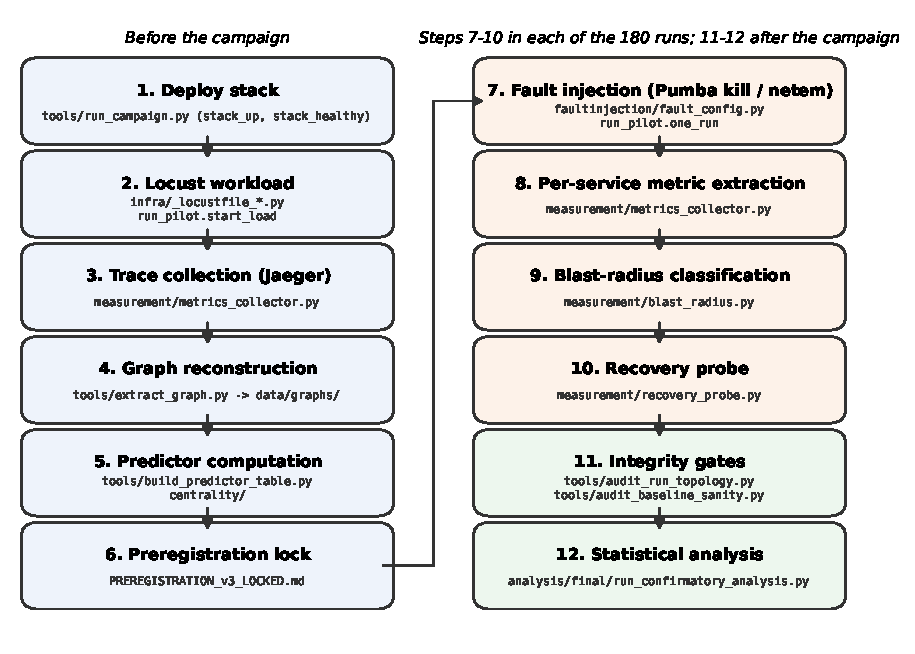
\includegraphics[width=\columnwidth]{generated/figures/fig_pipeline.pdf}
\caption{Pipeline in execution order. Each box names the repository files that carry out the
step; the steps from fault injection to the recovery probe repeat in every run.}
\label{fig:pipeline}
\end{figure}

\subsection{Testbed}
\label{sec:testbed}

All experiments ran on one host, configured as in Table~\ref{tab:tbl_ieee_testbed}. The
application stacks, Jaeger and Pumba ran as containers inside the virtual machine of Docker
Desktop's WSL2 backend, while the load generator and the campaign runner ran as host processes
(Fig.~\ref{fig:deployment}). The runner stops every stack before the campaign and brings up one
application at a time, so the two never shared the \val{testbed_docker_vm_gib}~GiB memory
ceiling of the virtual machine. The Social Network stack has \val{testbed_containers_sn}
containers and the Hotel Reservation stack \val{testbed_containers_hr}. Traces were collected
with Jaeger \val{version_jaeger}, one all-in-one instance per application with
\val{testbed_jaeger_storage} storage. The memory ceiling, host memory and container counts were
recorded on \val{testbed_vm_record_date}, before the campaign. The host operating system, CPU
and Docker Desktop version were queried on \val{testbed_measured_on}, after the campaign, and
Table~\ref{tab:tbl_ieee_testbed} marks them as measured.

\begin{table*}[!t]
\centering
\caption{Testbed and run protocol; host values marked as measured were queried after the campaign}
\label{tab:tbl_ieee_testbed}
\footnotesize
\setlength{\tabcolsep}{3pt}

\begin{tabular}{p{3.3cm}p{9.6cm}p{4.6cm}}
\toprule
\textbf{Item} & \textbf{Value} & \textbf{Source} \\
\midrule
Host OS & Microsoft Windows 11 Home Single Language (10.0.26300) & measured on 2026-10-20 \\
Host CPU & 12th Gen Intel(R) Core(TM) i7-1255U, 10 cores, 12 threads & measured on 2026-10-20 \\
Host RAM (GB) & 15.7 & recorded 2026-09-24 \\
Docker Desktop & 4.91.0, WSL2 backend & version measured on 2026-10-20 \\
Docker VM memory (GiB) & 7.598 (WSL2 default) & recorded 2026-09-24 \\
Docker client / Compose & 29.8.0 / 5.5.1 & client recorded 2026-10-18; Compose measured on 2026-10-20 \\
Containers per stack & Social Network 27, Hotel Reservation 24 & recorded 2026-09-24; one stack at a time \\
DeathStarBench commit & 6ecb097 & pinned upstream commit \\
Jaeger & 1.62.0 all-in-one, in-memory storage & compose override file \\
Pumba & ghcr.io/alexei-led/pumba, untagged image & version not recorded \\
Python & 3.13.2 & repository README \\
Python libraries & NumPy 2.1.2, pandas 2.2.3, SciPy 1.14.1, statsmodels 0.14.6, NetworkX 3.6.1, matplotlib 3.9.2 & repository README \\
Locust & 2.46.3; 25 users, spawn rate 10 users/s, 0.5 to 1.5 s between requests & runner and Locust files \\
Request mix, Social Network & compose post 3, home timeline 5, user timeline 2 & Locust task weights \\
Request mix, Hotel Reservation & search 6, reservation 2, user 2, recommendation 1 & Locust task weights \\
Load before the fault (s) & 60, also the baseline window & runner \\
Fault hold (s) & 30 & runner \\
Recovery probe (s) & poll 1, confirmation 5, lag 5, cap 180 & runner \\
Cooldown (s) & 20 & runner \\
\bottomrule
\end{tabular}
\end{table*}


\begin{figure}[!t]
\centering
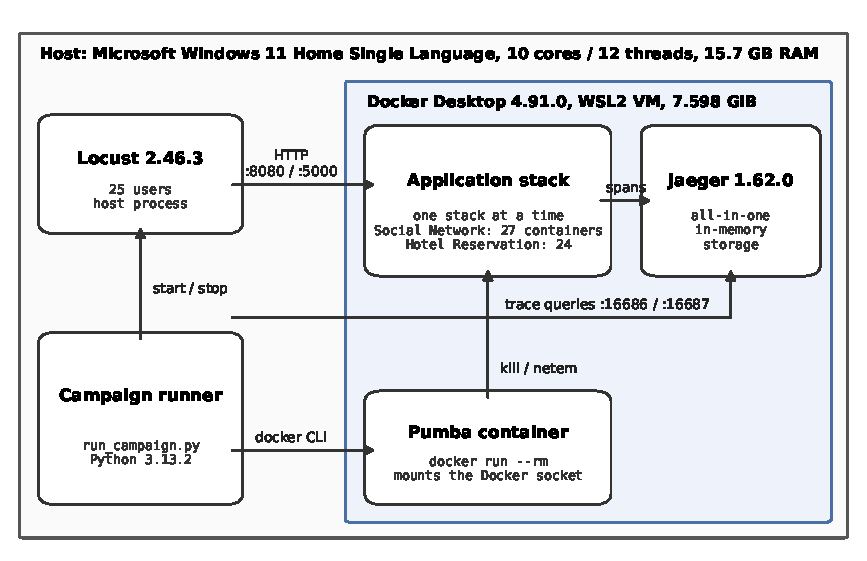
\includegraphics[width=\columnwidth]{generated/figures/fig_deployment.pdf}
\caption{Testbed deployment: the host, the Docker Desktop virtual machine with the application
stack, Jaeger and Pumba containers, and the Locust load generator and campaign runner on the
host.}
\label{fig:deployment}
\end{figure}

\subsection{Applications and Dependency Graphs}
\label{sec:apps}

Both applications come from DeathStarBench \cite{gan2019}, built from one pinned upstream
commit, \val{dsb_commit}, so the code under test was identical in every run. Their shapes
differ. Social Network is deep and fans out from a single composition service, while Hotel
Reservation is shallow and close to a star around its gateway. That difference turned out to
decide what each application could show (Section~\ref{sec:res-h1}).

The dependency graphs were taken from traces and not from documentation, because a diagram
shows the calls a system can make while the hypotheses concern the calls it makes under the
workload being perturbed. A directed edge runs from caller to callee wherever a span of one
service is the parent of a span of another \cite{sigelman2010}. The Social Network graph came
from \val{graph_sn_traces_examined} traces holding \val{graph_sn_spans_examined} spans, and
the Hotel Reservation graph from \val{graph_hr_traces_examined} traces holding
\val{graph_hr_spans_examined} spans. The graphs have \val{graph_sn_nodes} and
\val{graph_hr_nodes} services, with \val{graph_sn_edges} and \val{graph_hr_edges} observed call
edges (Figs.~\ref{fig:graph-sn} and~\ref{fig:graph-hr}). Both were frozen as files, and every
predictor is computed from those files.

\begin{figure}[!t]
\centering
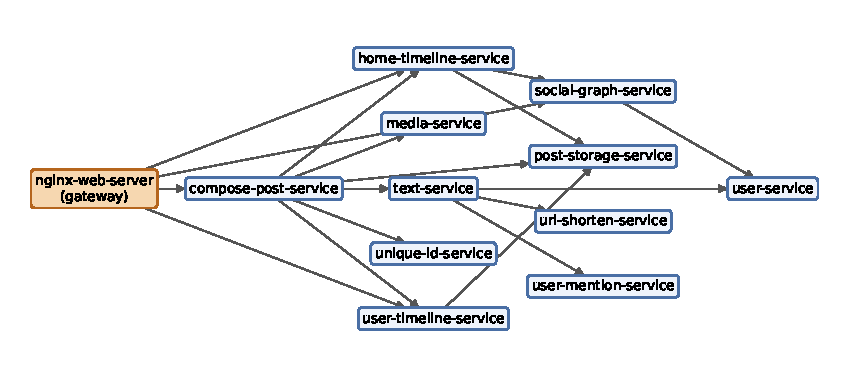
\includegraphics[width=\columnwidth]{generated/figures/fig_graph_sn.pdf}
\caption{Social Network dependency graph as observed in traces, with the gateway marked.}
\label{fig:graph-sn}
\end{figure}

\begin{figure}[!t]
\centering
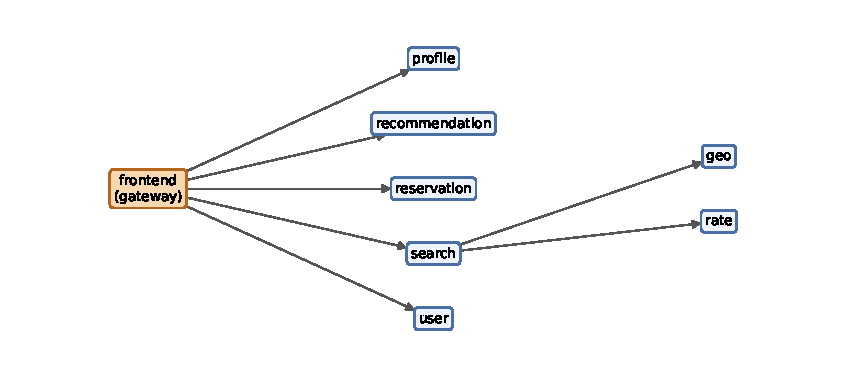
\includegraphics[width=\columnwidth]{generated/figures/fig_graph_hr.pdf}
\caption{Hotel Reservation dependency graph as observed in traces, with the gateway marked.}
\label{fig:graph-hr}
\end{figure}

The observed Hotel Reservation graph differs from the documented one. Of the
\val{hr_manifest_expected_edges} call edges implied by the published service tree, the traces
recover \val{hr_manifest_edges_recovered}. Two never appear under this workload,
%[id:hr_manifest_edges_missed]
\val{hr_manifest_edges_missed_names}, and one edge the tree does not list appears,
\val{hr_manifest_edges_extra}, which seems to stand in for the missing search-to-profile call.
The difference matters for one service: user has a single observed caller,
%[id:hr_user_observed_caller_count]
\val{hr_user_observed_callers}, where the documentation implies two. The observed graph is
used, and the divergence is reported.

\subsection{Analysis Set}
\label{sec:analysis-set}

Every correlation excludes the one service per application that has no caller in the graph:
nginx-web-server in Social Network and frontend in Hotel Reservation. A gateway receives
traffic only from the load generator, which is not a node of the graph, so its ancestor count
is zero by construction. Killing it also removes the only entry to the application and leaves
the outcome undefined. Without the gateways, \val{sn_services} services remain in Social
Network and \val{hr_services} in Hotel Reservation.

\subsection{Predictors}
\label{sec:predictors}

Section~\ref{sec:problem} defines the caller count and the hybrid metric. The ten further
comparators are degree, in-degree, out-degree, betweenness, closeness, eigenvector centrality
\cite{bonacich1987}, PageRank \cite{brin1998}, a composite rank, descendant count and dominator
subtree size, the number of services reachable from the gateway only through a given service.
Dominators are a classical notion for flow graphs \cite{lengauer1979}; here they are computed
with the immediate-dominator routine of NetworkX. Centralities follow the standard definitions
\cite{freeman1978}, and betweenness uses the algorithm of Brandes \cite{brandes2001}. The plan
forbade dropping any comparator after results were seen, and none was dropped.

The hybrid metric's weight values, \val{hybrid_w_in}, \val{hybrid_w_out} and
\val{hybrid_w_btw}, come from the project's original proposal, where an empirical search had
chosen them, so they were not fixed independently of all data. The locked plan called for tuning the weights on Social Network and
freezing them for Hotel Reservation. That step was never run (Deviation 10), and no weights were
re-tuned on campaign data. %[id:hybrid_weights_lockfile_exists] %[id:hybrid_weights_reoptimised_on_campaign]
A sensitivity analysis over every weighting on the preregistered grid, run after the
confirmatory results were known, is reported in Section~\ref{sec:res-weights}.
%[id:hybrid_weights_grid_evaluated_post_hoc]

Two predictor-application pairs were declared degenerate in advance because the predictor is
constant across the analysis set, which leaves Spearman's $\rho$ undefined. Eigenvector
centrality is zero for every analysed Social Network service, %[id:degenerate_sn_value]
since the reconstructed graph is acyclic, and every Hotel Reservation service has exactly one
direct caller, so in-degree is constant there. Both pairs are left out of the test family,
because a degenerate graph property is not a null result and counting it as one would dilute
the correction. That leaves \val{testable_pairs} testable pairs of the
\val{total_predictor_pairs} considered.

\subsection{Workload and Run Protocol}
\label{sec:protocol}

Each run starts the load generator, Locust \val{version_locust}, with
\val{protocol_load_users} users spawned at \val{protocol_spawn_rate} per second. Each simulated
user waits between \val{protocol_sn_wait_min_s} and \val{protocol_sn_wait_max_s} seconds
between requests %[id:protocol_hr_wait_min_s] %[id:protocol_hr_wait_max_s]
and draws each request from a fixed weighted mix (Table~\ref{tab:tbl_ieee_testbed}). On
Social Network the weights are \val{protocol_sn_task_weight_compose_post} for composing a post,
\val{protocol_sn_task_weight_read_home_timeline} for reading a home timeline and
\val{protocol_sn_task_weight_read_user_timeline} for reading a user timeline. On Hotel
Reservation they are \val{protocol_hr_task_weight_hotel_search} for a hotel search,
\val{protocol_hr_task_weight_make_reservation} for a reservation,
\val{protocol_hr_task_weight_get_user} for a user lookup and
\val{protocol_hr_task_weight_get_recommendations} for recommendations.

The load runs for \val{protocol_warmup_s} seconds before the fault, and the fault-free baseline
percentiles are computed over that same \val{protocol_baseline_window_s}-second window. The
window therefore opens when the load generator starts and includes its ramp-up (Deviation 13);
its length was the same in every run. %[id:protocol_baseline_window_distinct]
The fault is then held for \val{protocol_fault_duration_s} seconds, the recovery probe runs,
and a \val{protocol_cooldown_s}-second cooldown separates one run from the next.

Faults are injected with Pumba, which the runner starts as a short-lived container that acts on
the target container through the Docker socket; every command goes through the Docker
\val{version_docker_client} client. Table~\ref{tab:tbl_ieee_commands} lists the command lines,
generated from the runner code. A kill fault sends \val{fault_kill_signal}, which ends the
process without draining connections or answering requests in flight. A latency fault applies
a \texttt{tc netem} rule that adds \val{fault_latency_delay_ms}~ms of delay, with
\val{fault_latency_jitter_ms}~ms of jitter, to the container's network interface. The kill asks
what happens when a dependency vanishes; the delay asks what happens when it stays up but
answers late.

\begin{table*}[!t]
\centering
\caption{Command lines issued in each run, generated from the runner code}
\label{tab:tbl_ieee_commands}
\footnotesize
\setlength{\tabcolsep}{3pt}

\begin{tabular}{p{2.9cm}p{11.9cm}p{2.7cm}}
\toprule
\textbf{Step} & \textbf{Command} & \textbf{Source} \\
\midrule
Start the load & \texttt{python -m locust -f <locustfile> -{}-host <url> -{}-headless -{}-users <users> -{}-spawn-rate 10 -{}-run-time <duration>s -{}-only-summary -{}-loglevel ERROR} & runner, load start \\
Find the target container & \texttt{docker ps -{}-filter label=com.docker.compose.service=<service> -{}-format '\{\{.Names\}\}\textbackslash\{\}t\{\{.Label "com.docker.compose.service"\}\}'} & runner, target resolution \\
Kill fault & \texttt{docker run -{}-rm -v /var/run/docker.sock:/var/run/docker.sock ghcr.io/alexei-led/pumba kill -{}-signal SIGKILL <container>} & fault configuration \\
Latency fault & \texttt{docker run -{}-rm -v /var/run/docker.sock:/var/run/docker.sock ghcr.io/alexei-led/pumba netem -{}-duration 30s delay -{}-time 500 -{}-jitter 100 <container>} & fault configuration \\
Restore after a kill & \texttt{docker compose up -d <service>} & runner, restore \\
Clean up after a latency fault & \texttt{docker compose up -d -{}-force-recreate <service>} & runner, clean-up \\
\bottomrule
\end{tabular}
\end{table*}


The runner finds the target as the one container whose \texttt{com.docker.compose.service}
label equals the service name exactly, and it stops if none or several match, so that a fault
cannot land on a different service from the one recorded (Deviation 2). Timing differs by fault
type. A kill completes at once; the runner waits out the fault window, restores the service
with \texttt{docker compose up -d}, and takes the fault-removal instant when that command
returns. Because \texttt{pumba netem} blocks for its declared duration, the runner launches it
as a separate process and takes the fault-removal instant when that process exits. After the
recovery probe of every latency run, the runner recreates the target container so that no
residual netem rule reaches the next run (Deviation 4). Algorithm~\ref{alg:run} gives one run in
full, with warm-up and baseline window $W$ of \val{protocol_warmup_s}~s, fault hold $H$ of
\val{protocol_fault_duration_s}~s, probe interval $P$ of \val{trec_poll_interval_nominal_s}~s,
confirmation period $K$ of \val{protocol_confirm_s}~s, probe lag $L$ of
\val{protocol_probe_lag_s}~s and recovery cap $C$ of \val{protocol_recovery_cap_s}~s.

\begin{algorithm}[!t]
\caption{One campaign run (\texttt{one\_run} in \texttt{tools/run\_pilot.py}), called in
manifest order with a cooldown after each run}
\label{alg:run}
\begin{algorithmic}[1]
\Require application $a$, service $s$, fault type $f$, repetition $r$, graph $G$ of $a$
\State $c \gets$ the running container whose label \texttt{com.docker.compose.service}
equals the compose name of $s$; stop unless exactly one matches
\State start the Locust load against the gateway of $a$
\State wait $W$; $B \gets$ per-service baseline percentiles and error rates over the last $W$
\State $t_{\mathrm{inj}} \gets$ now; issue the Pumba command for $f$ on $c$
\Comment{kill: synchronous; latency: background process}
\State wait $H$; $t_{\mathrm{end}} \gets$ now
\State $D \gets$ services degraded in $[t_{\mathrm{inj}}, t_{\mathrm{end}}]$ relative to $B$
\State persist the raw spans of the baseline and fault windows
\If{$f = \text{kill}$}
  \State run \texttt{docker compose up -d} for $s$
\Else
  \State wait for the Pumba process to exit
\EndIf
\State $t_{\mathrm{rm}} \gets$ now \Comment{fault-removal instant}
\State $\Trec \gets$ recovery probe from $t_{\mathrm{rm}}$ with interval $P$, confirmation $K$,
lag $L$ and cap $C$
\If{$f \neq \text{kill}$}
  \State run \texttt{docker compose up -d -{}-force-recreate} for $s$
\EndIf
\State classify $D$ into ancestors, descendants and unrelated services of $s$ in $G$
\State stop the load; \Return the run record
\end{algorithmic}
\end{algorithm}

The design is fully crossed and balanced. Each analysable service receives each fault type
\val{campaign_reps_per_cell} times, giving \val{campaign_cells} cells and
\val{campaign_runs_total} runs, \val{sn_runs} on Social Network and \val{hr_runs} on Hotel
Reservation. A run with incomplete telemetry is discarded and repeated in its own cell; it is
never replaced elsewhere and never analysed as zeros. The same rule covered the
\val{deviations_runs_invalidated} runs invalidated by Deviations 1, 2 and 4, which were
collected again in their cells. %[id:deviation_1_runs_invalidated] %[id:deviation_2_runs_invalidated] %[id:deviation_4_runs_invalidated]
The campaign ran from \val{campaign_start_utc} to \val{campaign_end_utc} UTC, measured from the
first to the last end-timestamp of the kept runs, and lost \val{campaign_runs_failed} runs to
telemetry failure. The raw spans of the baseline and fault windows were stored for every run,
so any later change to a metric definition can be replayed on the original data without
repeating the experiment.

\subsection{Per-Service Latency and Error Attribution}
\label{sec:attribution}

The latency definition needed more care than any other part of the method, because the obvious
implementation is wrong in a way that is easy to miss. A tracing backend asked for the traces
involving a service returns every trace in which the service appears, and the root span of each
trace times the whole request from end to end. A percentile over those root spans, labelled as
the p95 of the service, is really the end-to-end p95 of every request that passed through it,
and every service on a request path receives the same value. Error rate has the same flaw if a
trace counts as failed whenever any of its spans carries an error. Services on a shared path
then become indistinguishable, and a threshold flags them as a group.

Fig.~\ref{fig:q3} shows the effect on Hotel Reservation under a latency fault in the search
service, using \val{q3_pilot_runs} pilot validation runs that are not part of the campaign.
Under the end-to-end scope, three services, %[id:q3_identical_baseline_services]
\val{q3_identical_baseline_names}, share an identical baseline p95 in both runs, and a
multiplicative threshold flags five services that were not faulted.
%[fig:fig_q3_artifact]
Two of them, profile and reservation, are neither ancestors nor descendants of search; they
share a trace with it and nothing more.

\begin{figure*}[!t]
\centering
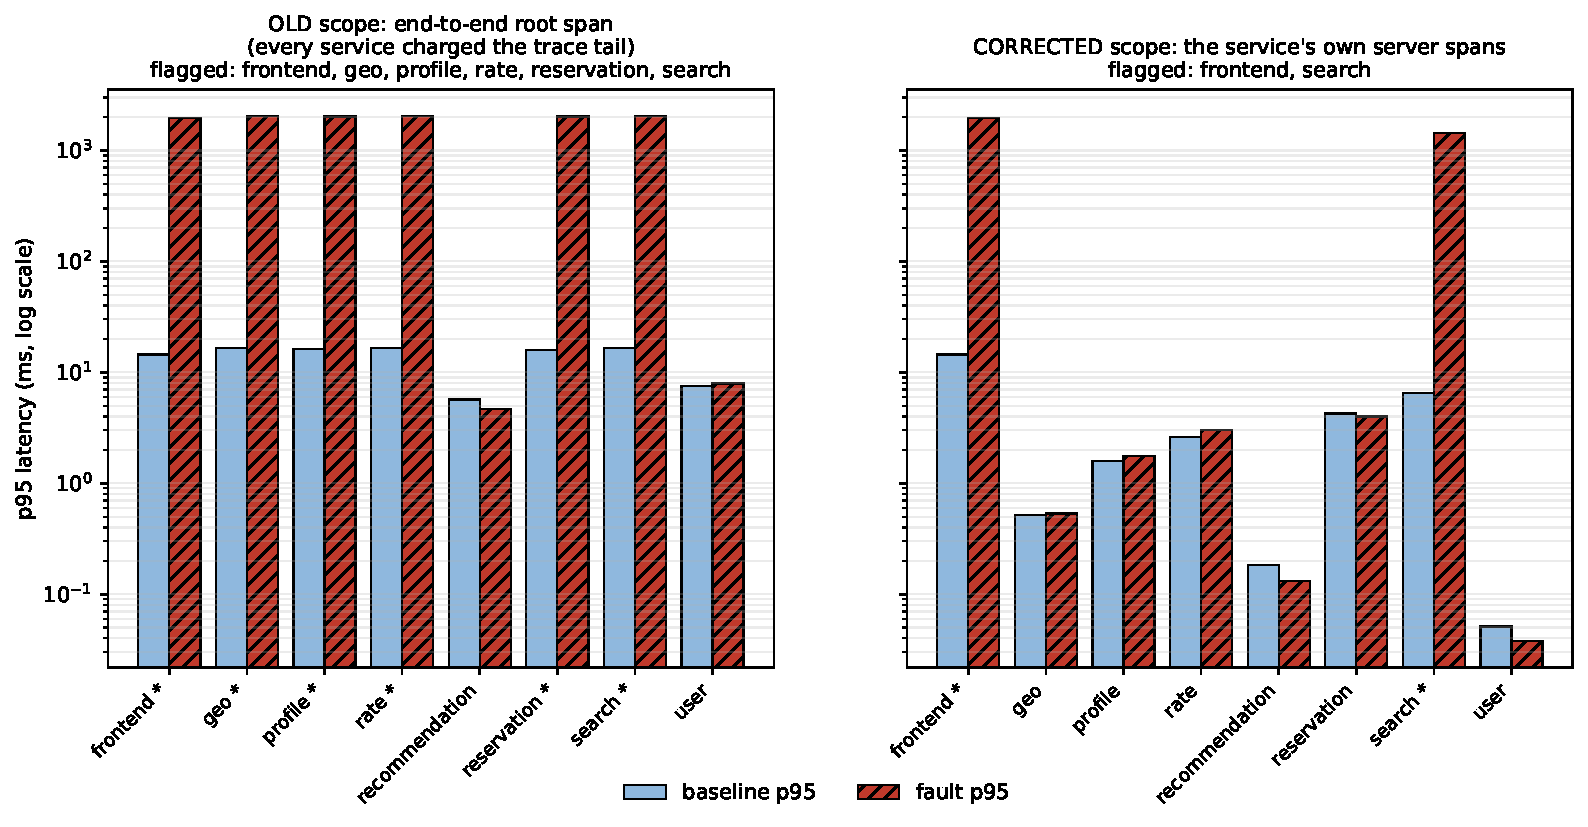
\includegraphics[width=0.82\textwidth]{generated/figures/fig_q3_artifact.pdf}
\caption{Per-service p95 on Hotel Reservation under a latency fault in search, measured on the
end-to-end root span of each trace (left) and on each service's own spans (right). An asterisk
marks a service flagged as degraded.}
\label{fig:q3}
\end{figure*}

Each service's latency is therefore measured on the spans that service emits itself. On Hotel
Reservation, whose spans carry a span-kind tag, client spans are excluded, because a client
span recorded by a service times its callee and would pass a downstream delay back up. Social
Network's spans carry no span-kind tag, so all of a service's spans were used there, and
\val{sn_spans_selected_client_pct}\% of the spans used were client spans. A post hoc replay
restricted to server spans changed the outcome of \val{replay_runs_changed} of \val{replay_runs}
runs and none of the service-level medians, and the primary result came out identical
(Deviation 11). %[id:replay_service_medians_changed] %[id:replay_primary_identical] %[id:sn_span_samples_fallback]
An error counts against a service only when one of its own spans is tagged as an error, divided
by the number of traces in which the service appears. With per-service attribution, the same
two pilot runs flag one non-faulted service instead of five, and that service is an ancestor of
search. %[fig:fig_q3_artifact]
The services that drop out keep a flat service time while the end-to-end value charged to them
grows more than a hundredfold, the signature of a measurement artifact; shared-resource
contention would raise their own service times.

\subsection{Outcomes: Blast Radius and Recovery Time}
\label{sec:outcomes}

A service counts as degraded when either of two conditions holds on its own spans during the
fault window. The latency condition requires its p95 to exceed
\val{threshold_degradation_factor}$\times$ its baseline p95 and to rise by at least
\val{threshold_degradation_floor_ms}~ms. The error condition requires its error rate to rise by
at least \val{threshold_error_rate_abs} in absolute terms. The absolute floor became necessary
once percentiles were truly per service: some services here have baseline p95 values in the
hundredths of a millisecond, where a purely multiplicative rule reacts to scheduler noise
(Deviation 1). Both conditions are evaluated at full precision. Degraded services are split
into the ancestor, descendant and unrelated counts of Section~\ref{sec:problem}.

Which indicator carries the signal depends on the fault type, and the plan fixed the pairing in
advance. Under kill faults the primary indicator is error rate, because requests fail; in the
pilot the sign of the kill-fault change in p95 even differed between the two applications, so
it is never pooled. Under latency faults the change in p95 is the primary indicator and error
rate carries no signal, because nothing has failed.

Recovery time, \Trec, is the number of seconds from fault removal until the changes in p95, p99,
error rate and downstream-affected count are all back within
\val{protocol_recovery_tolerance_pct}\% of their baseline and stay
there for a \val{protocol_confirm_s}-second confirmation period. Timing from removal matters,
since timing from injection would include the whole fault and could never fall below it. The
probe polls at a nominal \val{trec_poll_interval_nominal_s}-second interval, with an effective
resolution of \val{trec_poll_interval_eff_min_s} to \val{trec_poll_interval_eff_max_s} seconds
measured as the median gap between samples within each run. Each sample reads a window lagged
\val{protocol_probe_lag_s} seconds into the past, because tracing backends flush spans in
batches, and needs at least \val{protocol_min_traces} traces before its percentiles can vote for
recovery. A run that has not recovered within \val{protocol_recovery_cap_s} seconds is recorded
as right-censored and never filled in with a number. No run was censored.
%[id:campaign_runs_censored]
Observed recovery times ranged from \val{trec_min_s}~s to \val{trec_max_s}~s, with a median of
\val{trec_median_s}~s. The plan stated in advance that a low censoring rate would make the rank
test the primary test for \Trec, with survival models reported beside it; at a censoring rate of
\val{campaign_censoring_rate_pct}\%, that rule applied (Deviation 6).

\subsection{Statistical Analysis}
\label{sec:stats}

Associations between a graph predictor and a measured outcome are tested with Spearman's
$\rho$ at the service level, after taking the median over each service's repetitions; the
repetitions make each service's value more precise but add no points to the correlation.
Significance comes from permutation tests, exact where all orderings can be enumerated and
otherwise from \val{primary_n_permutations} random permutations, with one added to both counts
so that no p-value is zero \cite{phipson2010}. The asymptotic approximation is unreliable at
these sample sizes and with the ties these graphs produce. Confidence intervals are
bias-corrected and accelerated bootstrap intervals \cite{efron1987}, with a percentile interval,
marked as such, where ties leave the bias correction undefined. For recovery time the Cox
proportional hazards model \cite{cox1972} and the log-rank test serve as secondary analyses. The
analysis ran on Python \val{version_python}, with SciPy \val{version_scipy} supplying ranks and
the reference Spearman implementation and statsmodels \val{version_statsmodels} the survival
models.

Tests fall into three families, each corrected separately with the Benjamini-Hochberg
procedure at $q = \val{fdr_q}$ \cite{benjamini1995}. The confirmatory family holds
\val{conf_family_size} tests on kill faults: the \val{testable_pairs} testable pairs, each
against $Y$ and against \Trec. The replication family repeats them on latency faults.
%[id:repl_family_size]
A third, exploratory family covers secondary outcomes and carries no confirmatory weight. The
plan considered pooling the families into one correction and rejected it, because the
confirmatory and replication families ask the same question under different faults. Two gates
run before any statistic: one confirms that every expected service was present in every run,
and the other compares each run's fault-free baseline with those of all other runs, using the
median and the median absolute deviation. All \val{integrity_checks_total} pre-analysis
integrity checks passed. %[id:integrity_checks_passed]

\subsection{Preregistration and Deviations}
\label{sec:deviations}

The plan was locked before the campaign started \cite{nosek2018}, and every later change was
logged with its date and with whether campaign data had been analysed by then.
\val{deviations_total} deviations were recorded; Appendix~\ref{app:deviations} lists them.
\val{deviations_no_data} invalidated no data. The other \val{deviations_with_data} invalidated
\val{deviations_runs_invalidated} runs, each collected again in its own cell, so the final
dataset is complete and balanced. Deviation 1 added the absolute latency floor after the
pre-launch rehearsal, Deviation 2 replaced a substring match that had faulted the wrong
container, and Deviation 4 dealt with a netem rule that outlived its run and inflated later
baselines. The remaining deviations concern the analysis or its reporting: the rank test
becoming primary for recovery time, an asymptotic p-value quoted in the plan, exact p-values
reported only as supplementary, the weight tuning that was not run, the Social Network span
selection, and Deviation 13, found while this paper was written, which records that the
baseline window includes the load ramp-up; it invalidated no run, and the baseline gate found no
anomalies.

\section{Results}
\label{sec:results}

\subsection{Campaign Completion}

All \val{campaign_runs_total} planned runs completed across \val{campaign_cells} balanced
cells. No run was lost to telemetry failure, no gateway was faulted, and every recovery time
was observed. %[id:campaign_runs_failed] %[id:campaign_gateway_runs] %[id:campaign_runs_censored]
Tables~\ref{tab:tbl_ieee_predictors_sn} and~\ref{tab:tbl_ieee_predictors_hr} list the graph
predictors and the measured outcomes of every analysed service.

\begin{table*}[!t]
\centering
\caption{Social Network: graph predictors and measured service medians for each analysed service}
\label{tab:tbl_ieee_predictors_sn}
\scriptsize
\setlength{\tabcolsep}{3pt}
\resizebox{\textwidth}{!}{%
\begin{tabular}{lrrrrrrrrrrrrr}
\toprule
\textbf{Service} & \textbf{Ancestors} & \textbf{Descendants} & \textbf{In-degree} & \textbf{Out-degree} & \textbf{HC} & \textbf{Betweenness} & \textbf{Closeness} & \textbf{PageRank} & \textbf{Eigenvector} & \textbf{\makecell[lb]{Degraded\\ancestors\\(kill)}} & \textbf{\makecell[lb]{Degraded\\ancestors\\(latency)}} & \textbf{\makecell[lb]{\textit{T}\textsubscript{rec}\\kill (s)}} & \textbf{\makecell[lb]{\textit{T}\textsubscript{rec}\\latency (s)}} \\
\midrule
post-storage-service & 4 & 0 & 3 & 0 & 0.109 & 0.000 & 0.291 & 0.157 & 0.000 & 4 & 4 & 15.3 & 15.4 \\
user-service & 4 & 0 & 2 & 0 & 0.073 & 0.000 & 0.242 & 0.145 & 0.000 & 2 & 2 & 14.5 & 14.8 \\
social-graph-service & 3 & 1 & 2 & 1 & 0.081 & 0.014 & 0.205 & 0.098 & 0.000 & 3 & 3 & 15.0 & 15.4 \\
url-shorten-service & 3 & 0 & 1 & 0 & 0.036 & 0.000 & 0.136 & 0.080 & 0.000 & 3 & 3 & 16.1 & 15.2 \\
user-mention-service & 3 & 0 & 1 & 0 & 0.036 & 0.000 & 0.136 & 0.080 & 0.000 & 3 & 3 & 14.5 & 14.4 \\
home-timeline-service & 2 & 3 & 2 & 2 & 0.096 & 0.012 & 0.182 & 0.074 & 0.000 & 2 & 2 & 15.4 & 15.6 \\
media-service & 2 & 0 & 1 & 0 & 0.036 & 0.000 & 0.121 & 0.061 & 0.000 & 2 & 2 & 16.1 & 14.8 \\
text-service & 2 & 2 & 1 & 2 & 0.064 & 0.036 & 0.121 & 0.061 & 0.000 & 2 & 2 & 15.3 & 14.4 \\
unique-id-service & 2 & 0 & 1 & 0 & 0.036 & 0.000 & 0.121 & 0.061 & 0.000 & 2 & 2 & 14.2 & 14.6 \\
user-timeline-service & 2 & 1 & 2 & 1 & 0.079 & 0.003 & 0.182 & 0.066 & 0.000 & 2 & 2 & 15.7 & 14.9 \\
compose-post-service & 1 & 10 & 1 & 7 & 0.302 & 0.053 & 0.091 & 0.062 & 0.000 & 1 & 1 & 15.6 & 15.6 \\
\bottomrule
\end{tabular}}
\end{table*}

\begin{table*}[!t]
\centering
\caption{Hotel Reservation: graph predictors and measured service medians for each analysed service}
\label{tab:tbl_ieee_predictors_hr}
\scriptsize
\setlength{\tabcolsep}{3pt}
\resizebox{\textwidth}{!}{%
\begin{tabular}{lrrrrrrrrrrrrr}
\toprule
\textbf{Service} & \textbf{Ancestors} & \textbf{Descendants} & \textbf{In-degree} & \textbf{Out-degree} & \textbf{HC} & \textbf{Betweenness} & \textbf{Closeness} & \textbf{PageRank} & \textbf{Eigenvector} & \textbf{\makecell[lb]{Degraded\\ancestors\\(kill)}} & \textbf{\makecell[lb]{Degraded\\ancestors\\(latency)}} & \textbf{\makecell[lb]{\textit{T}\textsubscript{rec}\\kill (s)}} & \textbf{\makecell[lb]{\textit{T}\textsubscript{rec}\\latency (s)}} \\
\midrule
geo & 2 & 0 & 1 & 0 & 0.057 & 0.000 & 0.190 & 0.152 & 0.707 & 2 & 2 & 22.0 & 17.7 \\
rate & 2 & 0 & 1 & 0 & 0.057 & 0.000 & 0.190 & 0.152 & 0.707 & 2 & 2 & 20.9 & 16.9 \\
profile & 1 & 0 & 1 & 0 & 0.057 & 0.000 & 0.143 & 0.124 & 0.002 & 1 & 1 & 27.0 & 18.7 \\
recommendation & 1 & 0 & 1 & 0 & 0.057 & 0.000 & 0.143 & 0.107 & 0.002 & 1 & 1 & 22.6 & 25.4 \\
reservation & 1 & 0 & 1 & 0 & 0.057 & 0.000 & 0.143 & 0.127 & 0.002 & 1 & 1 & 19.3 & 16.6 \\
search & 1 & 2 & 1 & 2 & 0.112 & 0.048 & 0.143 & 0.119 & 0.002 & 1 & 1 & 22.3 & 24.7 \\
user & 1 & 0 & 1 & 0 & 0.057 & 0.000 & 0.143 & 0.119 & 0.002 & 1 & 1 & 19.7 & 13.6 \\
\bottomrule
\end{tabular}}
\end{table*}


\subsection{The Confirmatory Test of H1}
\label{sec:res-h1}

On Social Network under kill faults, the caller count $X$ and the number of degraded callers
$Y$ correlate at $\rho = \val{primary_rho}$ across \val{primary_n_services} services, with a
bias-corrected and accelerated bootstrap interval from \val{primary_ci_lo} to
\val{primary_ci_hi}. The uncorrected p-value from \val{primary_n_permutations} random
permutations is \val{primary_p_locked}. After Benjamini-Hochberg correction across the
\val{conf_family_size} tests of the confirmatory family, the adjusted p-value is
\val{primary_p_bh_locked}. Exact enumeration, run after the results were known (Deviation 9),
gives \val{primary_p_exact} uncorrected and \val{primary_p_bh_exact} adjusted, and the verdict
does not change.\footnote{The locked Monte Carlo values remain the preregistered result.}
%[id:primary_significant_exact] %[id:primary_ci_method]

Not one of the \val{conf_family_size} confirmatory tests reaches significance at
$q = \val{fdr_q}$.
%[id:conf_family_significant]
The primary test has the smallest uncorrected p-value in the family, %[id:conf_best_raw_p] %[id:conf_best_predictor]
and its adjusted value is about \val{primary_p_bh_over_q} times the threshold.
Table~\ref{tab:tbl_ieee_primary} gives the primary test for each family and application, and
Table~\ref{tab:tbl_ieee_families} summarises both families. H1 is not confirmed. The point
estimate is large and positive, the correction fixed in advance rejects it, and the interval
runs from no association to a perfect one.

\begin{table*}[!t]
\centering
\caption{Test of H1, caller count $X$ against degraded callers $Y$, in each family and application}
\label{tab:tbl_ieee_primary}
\scriptsize
\setlength{\tabcolsep}{3pt}

\begin{tabular}{lllrrllrp{2.3cm}rlp{2.0cm}}
\toprule
\textbf{Family} & \textbf{Fault} & \textbf{Application} & \textbf{Services} & \textbf{$\rho$} & \textbf{95\% CI} & \textbf{CI method} & \textbf{p (raw)} & \textbf{p method} & \textbf{p (BH)} & \textbf{Significant} & \textbf{Note} \\
\midrule
confirmatory & kill & Social Network & 11 & 0.785 & 0.000 to 1.000 & BCa & 0.0080 & Monte Carlo, 10,000 permutations & 0.3451 & no &  \\
confirmatory & kill & Hotel Reservation & 7 & 1.000 & 1.000 to 1.000 & percentile & 0.0476 & exact, 5,040 permutations & 0.3451 & no & saturated; directional only \\
replication & latency & Social Network & 11 & 0.785 & 0.000 to 1.000 & BCa & 0.0076 & Monte Carlo, 10,000 permutations & 0.1848 & no &  \\
replication & latency & Hotel Reservation & 7 & 1.000 & 1.000 to 1.000 & percentile & 0.0476 & exact, 5,040 permutations & 0.2328 & no & saturated; directional only \\
\bottomrule
\end{tabular}
\end{table*}

\begin{table*}[!t]
\centering
\caption{Family sizes and the number of tests that survive Benjamini-Hochberg correction}
\label{tab:tbl_ieee_families}
\footnotesize
\setlength{\tabcolsep}{3pt}

\begin{tabular}{llrrrrrp{5.0cm}}
\toprule
\textbf{Family} & \textbf{Fault} & \textbf{Tests} & \textbf{\makecell[lb]{Tests with\\defined p}} & \textbf{\makecell[lb]{Significant\\after BH}} & \textbf{\makecell[lb]{Smallest p\\(raw)}} & \textbf{Its p (BH)} & \textbf{Test with the smallest p} \\
\midrule
confirmatory & kill & 44 & 44 & 0 & 0.0080 & 0.3451 & Social Network, caller count \textit{X} against \textit{Y} \\
replication & latency & 44 & 44 & 0 & 0.0076 & 0.1848 & Social Network, caller count \textit{X} against \textit{Y} \\
\bottomrule
\end{tabular}
\end{table*}


Two features of the data qualify the estimate further, and they matter more than its p-value.
The first is saturation. Since $Y$ counts degraded callers and $X$ counts callers, $Y$ can never
exceed $X$, and if every service's measured count equalled its graph count the correlation
would be one by construction and would test nothing. On Hotel Reservation that is what
happened: each service's measured outcome matched its predictor in every run, under both fault
types. %[id:saturation_hr_kill_run] %[id:saturation_hr_kill_service] %[id:saturation_hr_latency_run]
Hotel Reservation is therefore tautological at the unit of analysis,
%[id:saturation_hr_kill_tautological]
and every Hotel Reservation result is reported as directional only.

Social Network is not fully saturated. Its run-level saturation under kill faults is
\val{saturation_sn_kill_run}, which is why $\rho$ falls short of one. Fig.~\ref{fig:primary}
shows the pattern: ten of the eleven services lie exactly on the line $y = x$.
%[id:saturation_sn_kill_service]
One departs from it. User-service has \val{userservice_ancestor_count} graph ancestors and
registered \val{userservice_measured} degraded ancestors in all \val{userservice_runs_departing}
of its kill repetitions. The empirical content of the Social Network correlation, as distinct
from its definitional content, rests on that one service. A leave-one-out recomputation,
designed after the confirmatory result was known and carrying no inferential weight, withholds
one service at a time (Fig.~\ref{fig:loo}). The correlation then ranges from
\val{loo_rho_min} to \val{loo_rho_max}, and the value of \val{loo_userservice_rho} comes from
withholding user-service.

\begin{figure*}[!t]
\centering
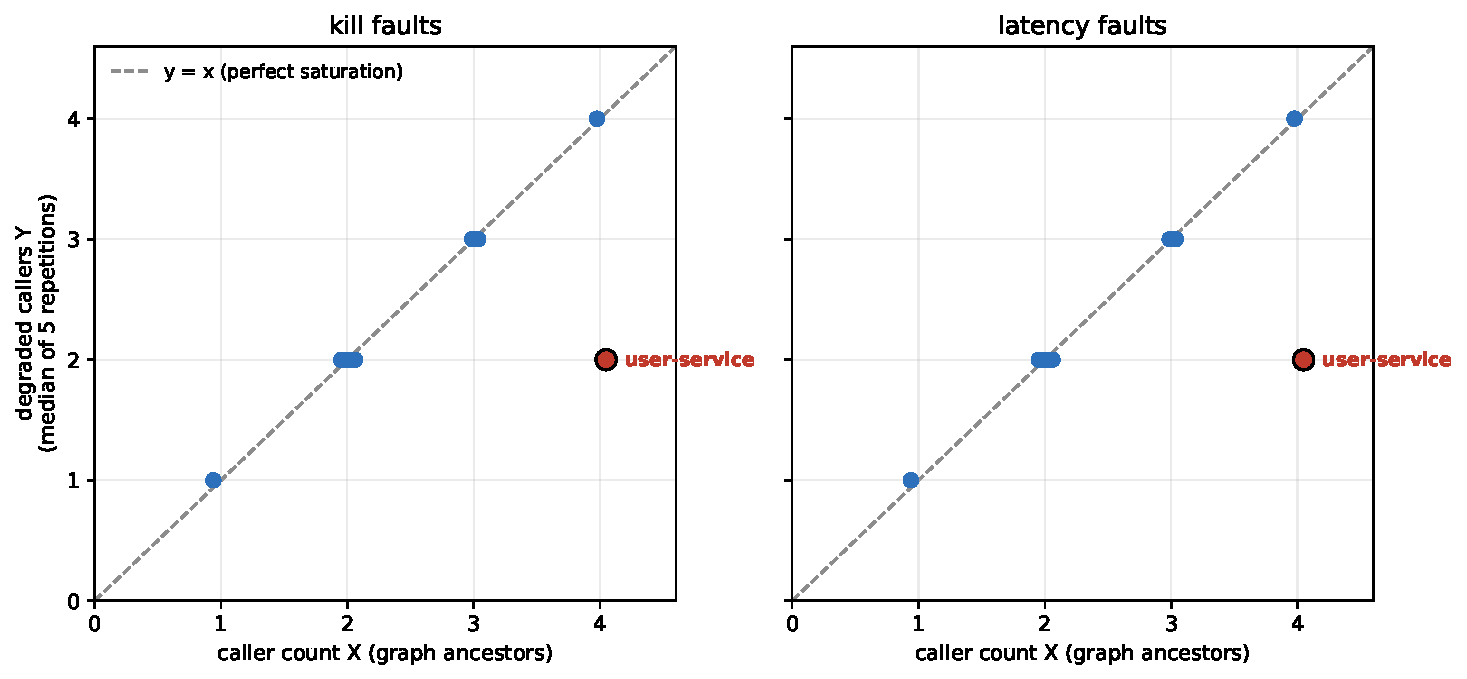
\includegraphics[width=0.78\textwidth]{generated/figures/fig_primary_sn.pdf}
\caption{Caller count $X$ against the measured number of degraded callers $Y$ for each Social
Network service under kill and latency faults. Points on the dashed line $y = x$ are
saturated; the labelled service departs from it.}
\label{fig:primary}
\end{figure*}

\begin{figure*}[!t]
\centering
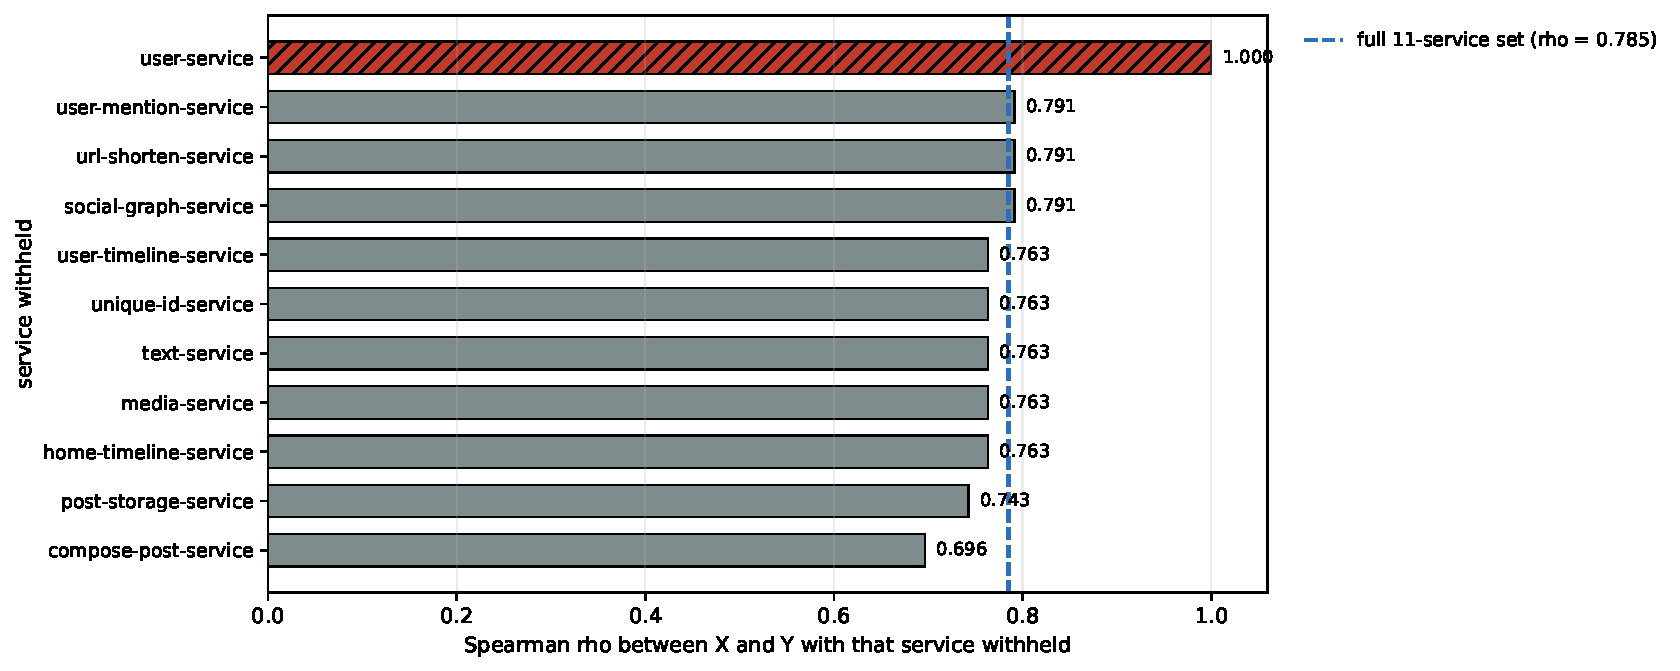
\includegraphics[width=0.78\textwidth]{generated/figures/fig_leave_one_out.pdf}
\caption{Post hoc leave-one-out check: Spearman's $\rho$ between $X$ and $Y$ on Social Network
under kill faults, recomputed with each service withheld.}
\label{fig:loo}
\end{figure*}

\subsection{The Hybrid Metric and H2}
\label{sec:res-h2}

The hybrid metric combines inbound centrality with a fan-out-scaled outbound term, on the
premise that a service calling many others matters because its failure breaks many downstream
links. H2 expected that premise to point the wrong way. Table~\ref{tab:tbl_ieee_h2} gives all
\val{h1b_cells} application and fault combinations. They are not independent: the outcome
vectors coincide across fault types, %[id:replication_primary_identical]
so the four cells hold \val{h1b_distinct_comparisons} distinct comparisons, one per application.

\begin{table*}[!t]
\centering
\caption{Test of H2, the hybrid metric HC against degraded callers $Y$, in all four application and fault cells}
\label{tab:tbl_ieee_h2}
\footnotesize
\setlength{\tabcolsep}{3pt}

\begin{tabular}{lllrrlrrlp{2.6cm}}
\toprule
\textbf{Family} & \textbf{Fault} & \textbf{Application} & \textbf{Services} & \textbf{$\rho$} & \textbf{95\% CI} & \textbf{p (raw)} & \textbf{p (BH)} & \textbf{$\rho$ $\leq$ 0} & \textbf{Distinguishable from zero after BH} \\
\midrule
confirmatory & kill & Social Network & 11 & \textminus{}0.144 & \textminus{}0.810 to 0.698 & 0.6688 & 0.9925 & yes & no \\
confirmatory & kill & Hotel Reservation & 7 & \textminus{}0.258 & \textminus{}0.730 to \textminus{}0.167 & 1.0000 & 1.0000 & yes & no \\
replication & latency & Social Network & 11 & \textminus{}0.144 & \textminus{}0.805 to 0.713 & 0.6656 & 0.9152 & yes & no \\
replication & latency & Hotel Reservation & 7 & \textminus{}0.258 & \textminus{}0.750 to \textminus{}0.167 & 1.0000 & 1.0000 & yes & no \\
\bottomrule
\end{tabular}
\end{table*}


The correlation between the hybrid metric and $Y$ is negative in every cell,
%[id:h1b_all_negative]
$\rho = \val{h1b_sn_kill_rho}$ on Social Network under both kill and latency faults
%[id:h1b_sn_latency_rho]
and $\rho = \val{h1b_hr_kill_rho}$ on Hotel Reservation. %[id:h1b_hr_latency_rho]
After correction no cell can be told apart from zero. %[id:h1b_any_distinguishable]
The adjusted p-values are \val{h1b_sn_kill_bh_p} and \val{h1b_sn_latency_bh_p} on Social
Network and \val{h1b_hr_kill_bh_p} on Hotel Reservation, %[id:h1b_hr_latency_bh_p]
and the Social Network interval runs from \val{h1b_sn_kill_ci_lo} to \val{h1b_sn_kill_ci_hi}.
The direction H2 states appears every time, but its size cannot be separated from zero, so no
negative relationship is claimed. What the data show is an absence of support for the fan-out
premise.

\subsection{The Motivating Case}

The metric was first motivated by compose-post-service, which calls
\val{composepost_out_degree} services directly and has \val{composepost_descendants}
transitive descendants. On the strength of that fan-out, the hybrid metric ranks it first of the
\val{composepost_set_size} analysed services, %[id:composepost_rank_hybrid]
with a score of \val{composepost_hybrid}. By transitive callers it ranks last, having a single
graph ancestor. %[id:composepost_rank_ancestor_count] %[id:composepost_ancestor_count]
Fig.~\ref{fig:rank} shows the full rank inversion.

\begin{figure}[!t]
\centering
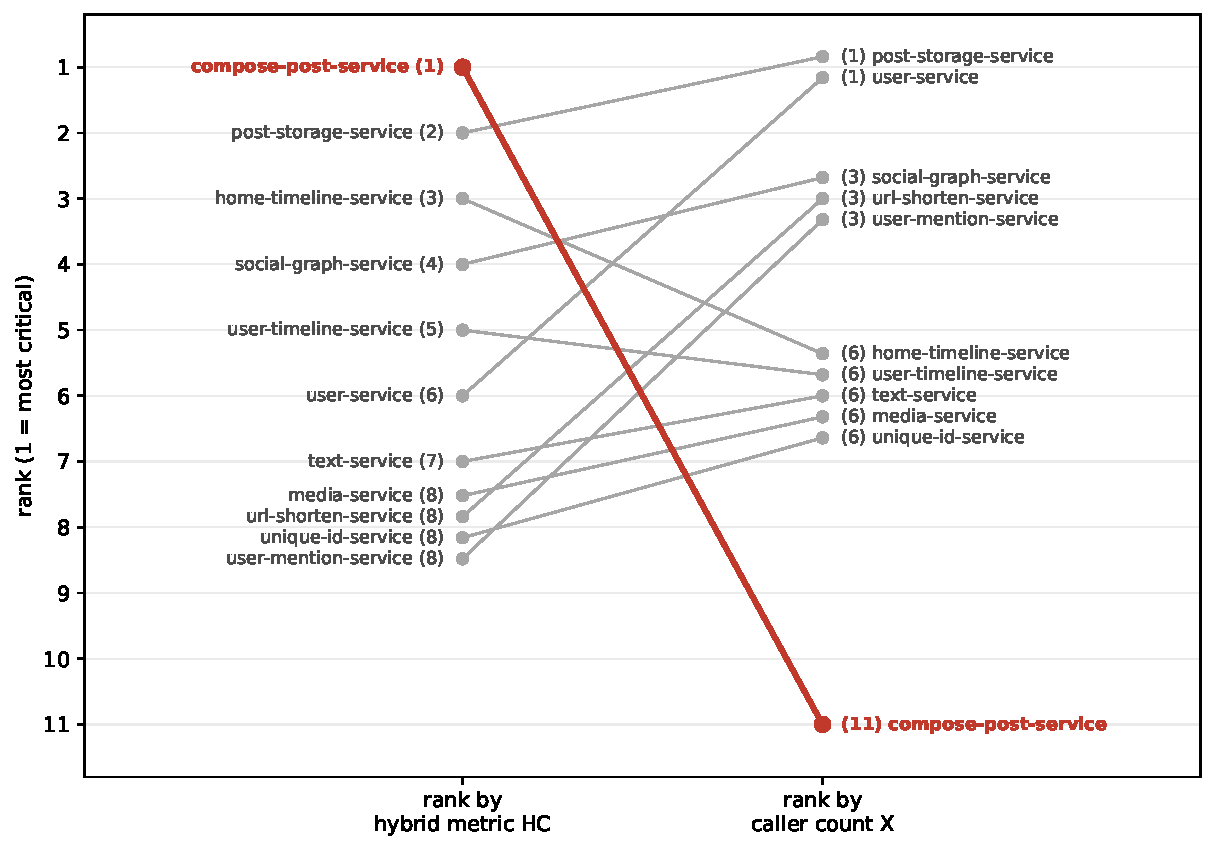
\includegraphics[width=\columnwidth]{generated/figures/fig_rank_inversion.pdf}
\caption{Rank of the eleven Social Network services by the hybrid metric HC and by caller
count $X$, with compose-post-service highlighted.}
\label{fig:rank}
\end{figure}

Measurement agrees with the caller-based ranking. Faulting compose-post-service left exactly
one degraded ancestor in each of its \val{composepost_kill_reps} kill repetitions,
%[id:composepost_kill_min] %[id:composepost_kill_max]
and the latency runs gave the same result. %[id:composepost_latency_min] %[id:composepost_latency_max]
A post hoc breakdown shows that in all \val{composepost_runs_total} runs that ancestor was
nginx-web-server, the gateway. %[id:composepost_runs_only_gateway_ancestor]
On the preregistered outcome, the service the original metric rates most critical is the lowest
in its application. The outcome counts degraded services, though, and does not measure requests
or functionality lost, and this is a single worked case: the test across all eleven services,
which could have generalised it, is the null result of Section~\ref{sec:res-h1}.

\subsection{Replication under a Second Fault Type}

The replication family repeats all \val{repl_family_size} tests on latency faults. Again no test
is significant after correction. %[id:repl_family_significant]
The smallest uncorrected p-value is \val{repl_best_raw_p}, with an adjusted value of
\val{repl_best_bh_p}. The agreement carries a caveat. Under kill and latency faults the service
medians of $Y$ are identical in both applications, %[id:replication_primary_identical]
and at run level \val{fault_invariant_services_all} of the
\val{fault_invariant_services_all_total} services show the same five per-run counts under both
fault types. On the primary outcome the latency family therefore repeats the kill family's
correlations on the same values and adds no independent evidence about H1.

Read on its own, this says that which services degrade when a service fails hardly depends on
how it fails: a process that disappears and a process that slows down reach the same
neighbours. Recovery differs. The correlation between median recovery times under kill and
under latency faults is \val{trec_rho_between_faults_sn} on Social Network and
\val{trec_rho_between_faults_hr} on Hotel Reservation, so for recovery time the second fault
type does add information.

\subsection{Direction of Propagation}
\label{sec:res-direction}

Across the campaign, degradation travelled to callers and not to callees. No descendant of the
faulted service degraded in \val{descendant_affected_runs_zero} of \val{campaign_runs_total}
runs, %[id:descendant_affected_runs_zero_pct]
and at the unit of analysis, the median over a service's repetitions, the count is zero for
every service under both fault types. %[id:descendant_affected_count_constant_at] %[id:descendant_affected_count_distinct_values]
The single exception, a kill repetition of compose-post-service on Social Network, recorded
\val{descendant_affected_max_in_any_run} degraded descendants.
%[id:descendant_affected_runs_nonzero] %[id:descendant_affected_exception_run]
Services unrelated to the faulted one behave the same way, with
\val{unrelated_affected_runs_zero} of \val{campaign_runs_total} runs at zero and one exception.
%[id:unrelated_affected_exception_run]

This is the firmest structural result of the study, and it cannot be written as a correlation.
Neither outcome varies between services, so \val{expl_undefined} of the \val{expl_attempted}
exploratory tests attempted have no defined value. A constant outcome gives no correlation at
all, which is different from a weak one. These tests are reported as undefined, with the
reason, in the same way as the \val{degenerate_pairs} degenerate predictors, and are not
entered as zeros.

\subsection{Exploratory Findings}

Of the \val{expl_testable} testable exploratory tests, \val{expl_significant} survive correction
within that family. Both concern the size of latency inflation under latency faults on Social
Network: the change in p95 correlates with the hybrid metric at
$\rho = \val{expl_sig_hybrid_criticality_rho}$ and with plain degree at
$\rho = \val{expl_sig_degree_rho}$, both with an adjusted p of
\val{expl_sig_hybrid_criticality_bh_p}. %[id:expl_sig_degree_bh_p]
These results carry no confirmatory weight, and their outcome is not the one H2 concerns. How
much latency inflates differs from how many callers degrade, and plain degree does at least as
well as the hybrid metric on it, which gives no reason to prefer the fan-out correction.

\subsection{What the Design Could Have Detected}
\label{sec:res-power}

Table~\ref{tab:tbl_ieee_power} reproduces the preregistered power analysis on the realised
analysis sets. Both sets have the registered size and the registered number of distinct
predictor values, and the ceiling correlations come out exactly as preregistered.
%[id:power_sn_n_matches] %[id:power_hr_n_matches] %[id:power_sn_levels_match] %[id:power_hr_levels_match] %[id:power_sn_ceiling_matches] %[id:power_hr_ceiling_matches]
The caller count takes only \val{power_sn_levels} distinct values across the
\val{power_sn_n} Social Network services and \val{power_hr_levels} across the \val{power_hr_n}
Hotel Reservation services. For an outcome without ties, these ties cap the attainable
correlation at \val{power_sn_ceiling} and \val{power_hr_ceiling}.

\begin{table}[!t]
\centering
\caption{Preregistered power analysis reproduced on the realised analysis sets; permutation p-values from 10000 random permutations (Social Network) and exact enumeration of 5040 permutations (Hotel Reservation)}
\label{tab:tbl_ieee_power}
\footnotesize
\setlength{\tabcolsep}{3pt}

\begin{tabular}{p{3.9cm}p{2.0cm}p{1.9cm}}
\toprule
\textbf{Quantity} & \textbf{Social Network} & \textbf{Hotel Reservation} \\
\midrule
Services, realised / preregistered & 11 / 11 & 7 / 7 \\
Distinct \textit{X} values, realised / preregistered & 4 / 4 & 2 / 2 \\
\textit{X} values & 1, 2, 2, 2, 2, 2, 3, 3, 3, 4, 4 & 1, 1, 1, 1, 1, 2, 2 \\
Ceiling $\rho$, outcome without ties, realised / preregistered & 0.941 / 0.941 & 0.791 / 0.791 \\
Ceiling p, outcome without ties, permutation & 0.0002 & 0.0952 \\
Ceiling p, outcome without ties, asymptotic (not for inference) & $<$0.0001 & 0.0343 \\
Ceiling $\rho$, outcome tied like \textit{X} & 1.000 & 1.000 \\
Ceiling p, outcome tied like \textit{X}, permutation & 0.0001 & 0.0476 \\
p quoted in the preregistration &  & 0.034 \\
\bottomrule
\end{tabular}
\end{table}


For Hotel Reservation the limit is severe. An outcome without ties can reach at best
$\rho = \val{power_hr_ceiling}$, with an exact permutation p of \val{power_hr_ceiling_p}, above
the conventional threshold before any correction. The preregistration quoted
\val{power_hr_prereg_stated_p} for this ceiling, which is the asymptotic value; the exact value
the plan requires is the one above (Deviation 7). Only an outcome that repeats the predictor's
own ties can do better, reaching $\rho = \val{power_hr_tied_rho}$ with p =
\val{power_hr_tied_p}, and saturation produced exactly that outcome
(Table~\ref{tab:tbl_ieee_primary}). Hotel Reservation could therefore pass the nominal threshold
before correction only by restating its predictor, and after correction its primary test is
far from significant. That follows from its tie structure and its size, not from anything
measured.

\subsection{Recovery Time}
\label{sec:res-trec}

No run was censored, so under the preregistered rule the Spearman rank test is the primary test
for recovery time, and the Cox and log-rank models are secondary and uncorrected (Deviation 6).
Table~\ref{tab:tbl_ieee_trec} gives all three for both predictors. No recovery-time test is
significant after correction in either family. %[id:trec_conf_significant] %[id:trec_repl_significant]
The log-rank test is undefined for \val{trec_conf_logrank_undefined} of the
\val{trec_conf_tests} recovery-time tests in each family, %[id:trec_repl_logrank_undefined] %[id:trec_repl_tests]
among them $X$ on Hotel Reservation, where the predictor has fewer than two distinct terciles.
Supplementary file S2 gives the unrounded estimates.

\begin{table*}[!t]
\centering
\caption{Recovery time: Spearman's $\rho$ (primary, BH-corrected within each family) and Cox and log-rank tests (secondary, uncorrected). Hazard ratios are per one-unit increase of the predictor, fitted per run with service-clustered errors and per service; the hybrid metric spans less than one unit, so its hazard ratios extrapolate beyond the observed range. Log-rank is undefined where the predictor has fewer than two distinct terciles}
\label{tab:tbl_ieee_trec}
\scriptsize
\setlength{\tabcolsep}{3pt}
\resizebox{\textwidth}{!}{%
\begin{tabular}{lllrrrrrrrrrr}
\toprule
\textbf{Fault} & \textbf{Application} & \textbf{Predictor} & \textbf{$\rho$} & \textbf{p (raw)} & \textbf{p (BH)} & \textbf{\makecell[lb]{HR per\\unit, run}} & \textbf{95\% CI, run} & \textbf{p, run} & \textbf{\makecell[lb]{HR per\\unit,\\service}} & \textbf{\makecell[lb]{95\% CI,\\service}} & \textbf{p, service} & \textbf{Log-rank p} \\
\midrule
kill & Social Network & caller count \textit{X} & \textminus{}0.356 & 0.2807 & 0.9264 & 1.173 & 0.876 to 1.570 & 0.2836 & 1.479 & 0.688 to 3.181 & 0.3163 & 0.5154 \\
kill & Social Network & hybrid metric HC & 0.098 & 0.7699 & 0.9925 & 0.010 & 0.002 to 0.043 & $<$0.0001 & 1.408 & $5.49\times10^{-4}$ to $3.61\times10^{3}$ & 0.9319 & 0.2099 \\
kill & Hotel Reservation & caller count \textit{X} & \textminus{}0.158 & 0.8571 & 0.9925 & 1.522 & 1.067 to 2.171 & 0.0204 & 2.179 & 0.302 to 15.722 & 0.4399 & undefined \\
kill & Hotel Reservation & hybrid metric HC & 0.204 & 0.8571 & 0.9925 & 0.147 & $8.91\times10^{-4}$ to 24.134 & 0.4609 & not estimable & not estimable & not estimable & undefined \\
latency & Social Network & caller count \textit{X} & \textminus{}0.060 & 0.8647 & 1.0000 & 0.998 & 0.816 to 1.221 & 0.9859 & 1.184 & 0.627 to 2.236 & 0.6018 & 0.5561 \\
latency & Social Network & hybrid metric HC & 0.767 & 0.0084 & 0.1848 & 0.045 & 0.002 to 1.163 & 0.0616 & $2.49\times10^{-4}$ & $8.19\times10^{-10}$ to 75.493 & 0.1975 & 0.1099 \\
latency & Hotel Reservation & caller count \textit{X} & \textminus{}0.158 & 0.8571 & 1.0000 & 0.882 & 0.578 to 1.346 & 0.5609 & 2.179 & 0.302 to 15.722 & 0.4399 & undefined \\
latency & Hotel Reservation & hybrid metric HC & 0.408 & 0.5714 & 0.8111 & $6.26\times10^{-4}$ & $1.07\times10^{-6}$ to 0.368 & 0.0234 & not estimable & not estimable & not estimable & undefined \\
\bottomrule
\end{tabular}}
\par\smallskip\parbox{\linewidth}{\scriptsize Not estimable: the Cox fit did not converge or showed separation because the predictor takes few distinct values; raw estimates are in supplementary file S2.}
\end{table*}


\subsection{Post Hoc Weight Sensitivity}
\label{sec:res-weights}

The confirmatory results were already in hand when this analysis was designed, and it belongs
to no preregistered family. It asks how much the hybrid metric's association with the outcome
depends on its weights. The metric was recomputed for all \val{ws_triplets} weight triplets on
the preregistered grid, with step \val{ws_grid_step} and weights summing to one, using the same
code, the same service medians and the same permutation tests. Each set of
\val{ws_triplets} tests was corrected with the Benjamini-Hochberg procedure within that set. No
triplet was selected or adopted, and every other result in this paper uses the reported
weights. Table~\ref{tab:tbl_ieee_weights} and Fig.~\ref{fig:weights} give the full distribution.

\begin{table*}[!t]
\centering
\caption{Post hoc weight sensitivity of the hybrid metric over 231 weight triplets, with BH correction within each set of 231}
\label{tab:tbl_ieee_weights}
\scriptsize
\setlength{\tabcolsep}{3pt}

\begin{tabular}{lllrrrrrrrrr}
\toprule
\textbf{Application} & \textbf{Fault} & \textbf{Outcome} & \textbf{\makecell[lb]{Triplets\\with\\defined $\rho$}} & \textbf{$\rho$ min} & \textbf{$\rho$ median} & \textbf{$\rho$ max} & \textbf{$\rho$ $>$ 0} & \textbf{\makecell[lb]{p (raw) $<$\\0.05}} & \textbf{\makecell[lb]{Significant\\after BH}} & \textbf{\makecell[lb]{$\rho$ at\\0.4/0.4/0.2}} & \textbf{\makecell[lb]{p at\\0.4/0.4/0.2}} \\
\midrule
Social Network & kill & degraded callers \textit{Y} & 231 & \textminus{}0.544 & \textminus{}0.167 & 0.337 & 28 & 0 & 0 & \textminus{}0.144 & 0.6695 \\
Social Network & latency & degraded callers \textit{Y} & 231 & \textminus{}0.544 & \textminus{}0.167 & 0.337 & 28 & 0 & 0 & \textminus{}0.144 & 0.6695 \\
Hotel Reservation & kill & degraded callers \textit{Y} & 230 & \textminus{}0.258 & \textminus{}0.258 & \textminus{}0.258 & 0 & 0 & 0 & \textminus{}0.258 & 1.0000 \\
Hotel Reservation & latency & degraded callers \textit{Y} & 230 & \textminus{}0.258 & \textminus{}0.258 & \textminus{}0.258 & 0 & 0 & 0 & \textminus{}0.258 & 1.0000 \\
Social Network & kill & gateway error rate & 231 & 0.229 & 0.753 & 0.832 & 231 & 145 & 128 & 0.786 & 0.0064 \\
Hotel Reservation & kill & gateway error rate & 230 & \textminus{}0.204 & \textminus{}0.204 & \textminus{}0.204 & 0 & 0 & 0 & \textminus{}0.204 & 0.8571 \\
\bottomrule
\end{tabular}
\end{table*}


\begin{figure}[!t]
\centering
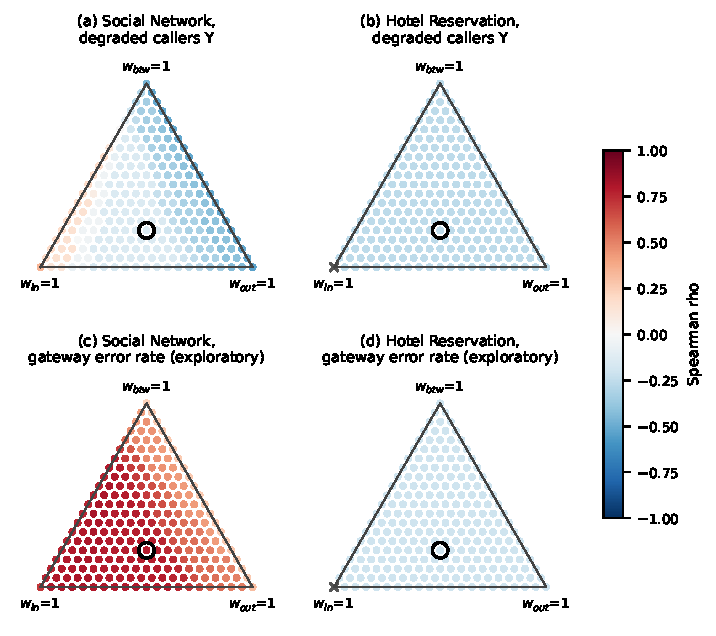
\includegraphics[width=\columnwidth]{generated/figures/fig_weight_sensitivity.pdf}
\caption{Post hoc weight sensitivity: Spearman's $\rho$ of the hybrid metric against degraded
callers (a, b) and the gateway error rate (c, d) for every weight triplet under kill faults;
latency faults give identical results for degraded callers. Circled: the reported weights;
cross: metric constant.}
\label{fig:weights}
\end{figure}

Against the number of degraded callers on Social Network, $\rho$ ranged from
\val{ws_sn_kill_anc_rho_min} to \val{ws_sn_kill_anc_rho_max}, with a median of
\val{ws_sn_kill_anc_rho_median}, and was positive for \val{ws_sn_kill_anc_triplets_rho_positive}
of the \val{ws_triplets} triplets. No triplet reached an uncorrected p below \val{fdr_q}; the
smallest was \val{ws_sn_kill_anc_p_raw_min}, %[id:ws_sn_kill_anc_triplets_p_raw_below_05]
and none survived correction. %[id:ws_sn_kill_anc_triplets_significant_bh]
Kill and latency faults gave identical results, since the service medians coincide.
%[id:ws_anc_identical_across_faults]
On Hotel Reservation every triplet with a defined correlation, \val{ws_hr_kill_anc_triplets_defined}
in all, gave $\rho = \val{ws_hr_kill_anc_rho_min}$, %[id:ws_hr_kill_anc_rho_max]
because a weighting on in-degree alone leaves the metric constant there.
%[id:ws_hr_kill_anc_triplets_undefined]
The reported weights gave $\rho = \val{ws_sn_kill_anc_reported_rho}$ on Social Network, and
\val{ws_sn_kill_anc_triplets_rho_above_reported} triplets gave a larger value. The null result
for H2 therefore does not hinge on the inherited weights: no weighting on the grid produced a
significant association with degraded callers in either direction.
%[id:ws_hr_kill_anc_triplets_significant_bh]

Against the gateway's error rate under kill faults, an exploratory outcome, the Social Network
picture differs. $\rho$ was positive for all \val{ws_sn_kill_err_triplets_rho_positive} triplets,
from \val{ws_sn_kill_err_rho_min} to \val{ws_sn_kill_err_rho_max} with a median of
\val{ws_sn_kill_err_rho_median}. Of these, \val{ws_sn_kill_err_triplets_p_raw_below_05} had
uncorrected p-values under \val{fdr_q}, and \val{ws_sn_kill_err_triplets_significant_bh}
remained significant after correction within the set; the p-values come from
\val{ws_mc_permutations} random permutations, because this outcome has too many distinct
orderings to enumerate. At the reported weights $\rho$ was \val{ws_sn_kill_err_reported_rho}.
The largest value is the best of \val{ws_triplets} tries on one dataset and is not a finding. On
Hotel Reservation every defined triplet gave $\rho = \val{ws_hr_kill_err_rho_min}$ and none was
significant. %[id:ws_hr_kill_err_triplets_significant_bh]
At the reported weights, the preregistered exploratory test of this association did not survive
correction across its exploratory family (adjusted $p = \val{uf_test_sn_hybrid_bh_p}$), and
Section~\ref{sec:disc-users} shows that the association follows the metric's in-degree term.

\subsection{Verification}

Two checks beyond the preregistered analysis are reported as supplementary. One is the post hoc
leave-one-out recomputation of Section~\ref{sec:res-h1}. The other is an independent
reimplementation of the primary statistic, written without reference to the analysis code and
reading only the stored spans and the dependency graph. It reproduces the reported correlation,
%[id:primary_rho_full]
and it agrees with the stored per-run outcomes on which services were affected, not only how
many, in all \val{sn_runs} Social Network runs. That shows the analysis code is faithful to its
data. Whether the definitions of Sections~\ref{sec:attribution} and~\ref{sec:outcomes} are the
right ones is a question no recomputation can settle.

\section{Discussion}
\label{sec:discussion}

\subsection{Why Fan-Out Points the Wrong Way}

The direction of propagation is the result that needs the fewest qualifications. In
\val{descendant_affected_runs_zero} of \val{campaign_runs_total} runs no descendant of the
faulted service degraded, and which services degraded hardly depended on how the fault was
delivered: for \val{fault_invariant_services_all} of the
\val{fault_invariant_services_all_total} services the per-run counts were identical whether the
service was killed or slowed down. The most plausible reading is that a caller suffers while it
waits on a dependency that has died or slowed, whereas a callee only receives fewer requests and
has nothing to wait for. The measurements fit that reading without testing it, because the
degradation rule asks only whether a service's own latency or error rate crossed a threshold and
never observes waiting directly.

If the reading is right, a fan-out ranking scores the wrong end of each edge. The composition
service of Social Network is the clearest case: it calls \val{composepost_out_degree} services
and the fan-out metric ranks it first, yet in each of its \val{composepost_runs_total} runs
exactly one caller degraded, and that caller was always the gateway.
%[id:composepost_runs_only_gateway_ancestor]
Across all services, the metric's correlation with degraded callers was negative in every cell
and separable from zero in none (Section~\ref{sec:res-h2}), and no weighting on the
preregistered grid changed that (Section~\ref{sec:res-weights}). The data give the fan-out
premise no support; they cannot show a negative relationship.

\subsection{A Predictor That Sits Close to Its Outcome}

The caller count correlates with degraded callers partly by construction, since the outcome
counts a subset of the predictor, and the two are equal whenever every ancestor of a faulted
service degrades. That held for every Hotel Reservation service and for ten of the eleven
Social Network services. %[id:saturation_hr_kill_service] %[id:saturation_sn_kill_service]
A post hoc breakdown sharpens the point. In all \val{gw_runs_all} runs the gateway was among the
degraded ancestors, %[id:gw_runs_gateway_degraded_all]
and in both applications every analysable service has the gateway among its graph ancestors.
%[id:gw_sn_services_gateway_ancestor] %[id:gw_hr_services_gateway_ancestor]
Every measured ancestor count therefore includes one unit that is the same for every service,
and what remains to be explained comes from intermediate callers. In Social Network only
user-service departs from its graph count in a consistent way. Its two ancestors that degraded
sit on request paths the workload exercises, and its other two showed no degradation in any run,
an explanation formed after seeing the data and not tested here.

With user-service withheld, the Social Network correlation becomes \val{loo_userservice_rho}.
The result can fairly be read as resting on one service's worth of independent information. One
lesson may reach beyond this study: a structural predictor tested against a structurally defined
outcome needs a saturation measure reported next to the correlation, without which the
correlation cannot be interpreted.

\subsection{What Users Would See}
\label{sec:disc-users}

The preregistered outcome counts degraded services and says nothing about how many requests
fail. To come closer to what a user experiences, the gateway's end-to-end error rate under kill
faults was examined after the fact. This analysis is exploratory and descriptive.

Gateway error followed the request mix. For each faulted service, the Locust task weights of the
request types whose traces pass through it were summed and divided by the total weight. The rank
correlation between that share and the median gateway error was
\val{uf_sn_rho_err_weight_share} on Social Network and \val{uf_hr_rho_err_weight_share} on
Hotel Reservation, reported without p-values. In Hotel Reservation, killing reservation, which
sits on request types carrying \val{uf_hr_reservation_weight_share} of the weight, gave a median
gateway error rate of \val{uf_hr_reservation_err_median}, while killing recommendation, with a
share of \val{uf_hr_recommendation_weight_share}, gave \val{uf_hr_recommendation_err_median}.
The mix does not explain everything. The Social Network services reached only through the
compose request all share a weight of \val{uf_sn_compose_post_service_weight_share}, and their
median error rates still range from \val{uf_sn_unique_id_service_err_median} to
\val{uf_sn_compose_post_service_err_median}.

The hybrid metric's exploratory correlation with gateway error on Social Network was
\val{uf_test_sn_hybrid_rho}, not significant after correction within its family (adjusted
$p = \val{uf_test_sn_hybrid_bh_p}$). Splitting the metric into its weighted terms shows where
the association comes from: the in-degree term alone has a rank correlation of
\val{uf_sn_rho_err_term_in} with gateway error, the fan-out term \val{uf_sn_rho_err_term_fanout}
and the betweenness term \val{uf_sn_rho_err_term_btw}. The association follows the count of
direct callers more closely than the fan-out correction, so it lends that correction no support.

\subsection{Lessons about Measurement}

Two measurement choices mattered more than the plan anticipated. The first is where latency is
attributed. Charging each trace's end-to-end latency to every service on the trace makes services
on a shared path indistinguishable; in the pilot comparison of Section~\ref{sec:attribution} that
shortcut flagged five non-faulted services where per-service attribution flagged one.
%[fig:fig_q3_artifact]
The correction was in place before the campaign, so what an uncorrected campaign would have
concluded is unknown, but the pilot shows how it would have behaved.

The second is that per-service attribution is only as good as the instrumentation behind it.
Social Network's spans carry no span-kind tag, so its per-service latency drew on all of a
service's spans, \val{sn_spans_selected_client_pct}\% of them client spans. A post hoc replay on
server spans altered \val{replay_runs_changed} of the \val{replay_runs} run outcomes and none of
the service-level medians. %[id:replay_service_medians_changed]
The change was small, which was fortunate. A study that depends on span semantics should check
them before collecting data, and this one did not.

\subsection{Implications for Practitioners}

For a team that has to rank services before running any experiment, the data favour looking up
the graph at callers over looking down it at callees. That advice rests on the propagation
pattern and on the lack of support for fan-out; the preregistered test of the caller ranking
itself did not reach significance, so no claim is made that it predicts failure impact. In both
applications the gateway appeared in every caller count, and in the exploratory analysis the
user-visible error rate tracked how much traffic passed through the failed service. A ranking
that weights callers by the traffic they carry may therefore be worth testing as a new
preregistered hypothesis; it was not tested here. Larger applications would also lift the
ceiling that eleven services place on any correlation, and containment mechanisms such as retries
with back-off or circuit breakers, which were neither configured nor studied, could change how
far a failure travels.

\section{Threats to Validity}
\label{sec:threats}

\subsection{Sample Size and Ties}

The unit of analysis is the service, so the sample sizes are \val{power_sn_n} for Social Network
and \val{power_hr_n} for Hotel Reservation, the number of services the applications have. Both
were registered in advance and matched exactly. %[id:power_sn_n_matches] %[id:power_hr_n_matches]
Repetition makes each service's outcome more precise, which is why each cell was run
\val{campaign_reps_per_cell} times, but it adds no points to a correlation. Ties tighten the
bound further: the caller count takes \val{power_sn_levels} distinct values on Social Network
and \val{power_hr_levels} on Hotel Reservation, which caps the correlation for an outcome
without ties at \val{power_sn_ceiling} and \val{power_hr_ceiling}. These ceilings were stated
before data collection, so they are a property of the design and not an explanation found
afterwards. On Hotel Reservation the outcome was also fully saturated, so every result there
restates how the outcome was built and is reported as directional only.
%[id:saturation_hr_kill_tautological]
Its value is as a second, differently shaped topology on which the direction result also holds.

\subsection{A Predictor Close to Its Outcome}

The most serious threat to the primary result is conceptual. The outcome counts degraded
transitive callers and the predictor counts transitive callers, so they coincide whenever every
ancestor degrades, and on Social Network the whole gap between $\rho = \val{primary_rho}$ and a
correlation of one rests on user-service. Withholding it raises $\rho$ to
\val{loo_userservice_rho}, a change \val{loo_swing_ratio} times the size of the next largest,
in a check specified after the result was known. The saturation measure was registered before
collection precisely to detect this, and the test remained meaningful because saturation was
not guaranteed in advance and did not fully hold. A reader may still treat the Social Network
correlation as one service's worth of evidence.

\subsection{Benchmarks, Workload and Graph}
\label{sec:threat-scope}

Both applications come from one benchmark suite at one commit, chosen because they are
instrumented and reproducible, not because they sample the space of microservice architectures.
The workload is synthetic, fixed at \val{protocol_load_users} users with a fixed request mix,
and containment mechanisms were not studied. Nothing here describes production behaviour.
Because the dependency graph is rebuilt from observed traffic, it is a property of deployment and
workload together; production call graphs change from request to request \cite{luo2021}. Even
here, the traces recover \val{hr_manifest_edges_recovered} of the
\val{hr_manifest_expected_edges} edges implied by Hotel Reservation's documentation, and the user
service has one observed caller where the documentation implies two.
%[id:hr_user_observed_caller_count]
A different request mix would give it a different predictor value with nothing about the
deployed system changed, which limits how far any relationship reported here carries to other
traffic.

\subsection{Measurement}

For latency faults, the runner infers that the netem rule is gone from the exit of the injecting
process. That inference failed at least once (Deviation 4). The cross-run baseline gate added
afterwards catches a rule that outlives its run, because later baselines then look contaminated,
but a rule that leaked and cleared within a single run would pass unnoticed, so latency-fault
recovery times carry an assumption the instrumentation cannot check. Blast-radius counts are
less exposed, since they come from the fault window itself. The server-span replay of
Deviation 11 could not cover recovery times on Social Network, because the probe's windows were
not stored, and those times stand as measured. The baseline window includes the load ramp-up (Deviation 13); the same
procedure ran in every run and the baseline gate reported no exceptions,
%[id:integrity_checks_passed]
but the size of any start-up effect was not measured. Two fault types were studied, a process
kill and a \val{fault_latency_delay_ms}~ms delay; CPU contention was evaluated in the pilot and
dropped because its effect was too small to classify reliably. Finally, some testbed values in
Table~\ref{tab:tbl_ieee_testbed} were queried after the campaign, on \val{testbed_measured_on},
and no record from the campaign days confirms that the host operating system build and Docker
Desktop version were unchanged.

\section{Conclusion}
\label{sec:conclusion}

A preregistered fault-injection campaign of \val{campaign_runs_total} balanced runs on two
benchmark applications asked whether a service's position in its dependency graph indicates how
much damage its failure does. The design crossed every analysable service with two fault types
and \val{campaign_reps_per_cell} repetitions, and the analysis was locked before the first run.

The correlational hypothesis did not survive. The number of transitive callers correlated
strongly with the number of degraded callers on Social Network, but after correction no test
survived in either family, the \val{conf_family_size} confirmatory and the
\val{repl_family_size} replication tests alike. %[id:conf_family_significant] %[id:repl_family_significant]
The fan-out-weighted metric this project began with correlated negatively in every cell
%[id:h1b_all_negative]
and could not be separated from zero in any, %[id:h1b_any_distinguishable]
and a post hoc sweep over \val{ws_triplets} weightings found none with a significant
association with degraded callers. %[id:ws_sn_kill_anc_triplets_significant_bh] %[id:ws_hr_kill_anc_triplets_significant_bh]

What held is structural. Failures reached callers and almost never callees: no descendant
degraded in \val{descendant_affected_runs_zero} of \val{campaign_runs_total} runs, and the
service-level median was zero in every condition. %[id:descendant_affected_count_constant_at]
That result needs no inference, and it held in both applications and under both fault types.

For practitioners, the evidence points towards ranking services by their callers and away from
ranking them by fan-out, with the caveat that the study's own test of the caller ranking did not
reach significance. For researchers, it shows two steps that are easy to skip: attributing
latency to each service's own spans, and measuring how far an outcome merely restates a
structural predictor before reporting a correlation between them. Every number in this paper can
be regenerated from the logged campaign data.


\section*{Data Availability}
The code, the raw campaign data (trace spans for every run, run records and the reconstructed
dependency graphs) and the analysis outputs are available at
\url{https://github.com/Daxx133-bot/proj-1-updated} and will be archived at Zenodo (DOI: [TO
FILL]). A single build script regenerates every number, table and figure in this paper from
the logged data. Three supplementary files accompany the paper in the repository: S1, the
leave-one-out recomputation of Section~\ref{sec:res-h1}
(\texttt{paper/tables/tbl\_leave\_one\_out.csv}); S2, the unrounded recovery-time estimates of
Section~\ref{sec:res-trec} (\texttt{paper/tables/tbl\_trec\_supplementary.csv}); and S3, the
exact-enumeration p-values for the confirmatory family
(\texttt{analysis/final/exact\_p\_supplement.csv}). Code is released under the MIT licence,
and data and figures under CC BY 4.0.

\section*{Acknowledgment}
The authors used an AI assistant (Claude, Anthropic) for code development support and
language editing. The authors performed all experiments and verified all content.

\bibliographystyle{IEEEtran}
\bibliography{generated/references}

\appendices
\section{Deviations from the Preregistered Plan}
\label{app:deviations}
Table~\ref{tab:tbl_ieee_deviations} lists every departure from the locked plan with its date,
the runs it affected and the action taken; Section~\ref{sec:deviations} summarises them. The
repository holds the full record, with a description of each deviation and of the change made.
\begin{table*}[!t]
\centering
\caption{Deviations from the preregistered plan}
\label{tab:tbl_ieee_deviations}
\footnotesize
\setlength{\tabcolsep}{3pt}

\begin{tabular}{rlp{6.4cm}rp{6.6cm}}
\toprule
\textbf{No.} & \textbf{Date} & \textbf{Deviation} & \textbf{\makecell[lb]{Runs\\affected}} & \textbf{Action} \\
\midrule
1 & 2026-09-26 & Absolute floor added to the latency rule & 3 & Floor added; rehearsal runs discarded \\
2 & 2026-09-26 & Wrong container targeted by a substring match & 3 & Exact label matching; affected runs collected again \\
3 & 2026-09-26 & Name mismatch stopped the campaign on a healthy stack & 0 & Stack check corrected; no data affected \\
4 & 2026-09-26 & Network-delay rule outlived its run & 11 & Affected runs collected again; container recreated after each latency run \\
5 & 2026-09-27 & Two choices the plan left open & 0 & Settled before the analysis was written \\
6 & 2026-09-27 & No run censored & 0 & Rank test made primary for recovery time as the plan required \\
7 & 2026-09-27 & Asymptotic p-value quoted in the plan & 0 & Exact value used \\
8 & 2026-09-27 & Statistical routines vectorised & 0 & Tested against the reference implementation \\
9 & 2026-09-28 & Exact p-values computed after the results & 0 & Reported as supplementary; verdict unchanged \\
10 & 2026-10-06 & Weight-tuning step not run & 0 & Inherited weights kept; not re-tuned \\
11 & 2026-10-06 & Social Network latency drew on all spans & 0 & Server-only replay; no service-level change \\
12 & 2026-10-06 & One latency run attempted twice & 0 & Only the completed attempt analysed \\
13 & 2026-10-20 & Baseline window includes the load ramp-up & 0 & Disclosed; baseline gate found no anomalies \\
\bottomrule
\end{tabular}
\end{table*}


\begin{IEEEbiographynophoto}{Dakshrajsinh Tank}
is a B.Tech student with the School of Computer Science and Engineering (SCOPE), Vellore
Institute of Technology, Vellore, India. [TO FILL: photograph and biography]
\end{IEEEbiographynophoto}

\begin{IEEEbiographynophoto}{Badrinath N}
is an Assistant Professor with the School of Computer Science and Engineering (SCOPE), Vellore
Institute of Technology, Vellore, India. [TO FILL: photograph and biography]
\end{IEEEbiographynophoto}

\end{document}
